%% Package and Class "uiucthesis2014" for use with LaTeX2e.
\documentclass[edeposit,fullpage,hidelinks]{uiucthesis2018}


\usepackage[acronym,toc]{glossaries}
\newacronym{MOSART}{MOSART}{the Molten Salt Actinide Recycler and Transmuter reactor}
\newacronym{PIE}{PIE}{postulated initiating event}
\newacronym{DBA}{DBA}{design basis accident}
\newacronym{MPK}{MPK}{modified point kinetics}
\newacronym{CFD}{CFD}{computational fluid dynamics}
\newacronym{DPK}{DPK}{delayed point reactor kinetics}
\newacronym{MSR}{MSR}{fluid-fueled molten salt reactor}
\newacronym{TFM}{TFM}{Transient Fission Matrix}
\newacronym{MSRs}{MSRs}{fluid-fueled molten salt reactors}
\newacronym{RELAP}{RELAP}{the Reactor Excursion and Leak Analysis Program}
\newacronym{SNM}{SNM}{special nuclear material}
\newacronym{ARISE}{ARISE}{Advanced Reactor International Safeguards Engagement}
\newacronym{TRANSFORM}{TRANSFORM}{Transient Simulation Framework of Reconfigurable Models}
\newacronym{TRU}{TRU}{trans-uranics}
\newacronym{LWR}{LWR}{light water reactor}
\newacronym{MSBR}{MSBR}{Molten Salt Breeder Reactor}
\newacronym{MSDR}{MSDR}{Molten Salt Demonstration Reactor}
\newacronym{MSFR}{MSFR}{Molten Salt Fast Reactor}
\newacronym{MOOSE}{MOOSE}{Multiphysics Object-Oriented Simulation Environment}
\newacronym{PP}{PP}{physical protection}
\newacronym{PR}{PR}{proliferation resistance}
\newacronym{IAEA}{IAEA}{International Atomic Energy Agency}
\newacronym{MSTDB-TC}{MSTDB-TC}{Molten Salt Thermodynamics Database - Thermochemical}
\newacronym{BlueCRAB}{BlueCRAB}{Comprehensive Reactor Analysis Bundle}
\newacronym{DNP}{DNP}{delayed neutron precursor}
\newacronym{FP}{FP}{fission product}
\newacronym{PRK}{PRK}{point reactor kinetics}
\newacronym{ODE}{ODE}{ordinary differential equation}
\newacronym{ADDER}{ADDER}{Advanced Dimensional Depletion for Engineering of Reactors}
\newacronym{MCNP}{MCNP}{Monte Carlo N-Particle}
\newacronym{DOE}{DOE}{Department of Energy}
\newacronym{MCA}{MCA}{material control and accountability}
\newacronym{HEU}{HEU}{highly enriched uranium}
\newacronym{LEU}{LEU}{low enriched uranium}
\newacronym{MSRE}{MSRE}{Molten Salt Reactor Experiment}
\newacronym{SAM}{SAM}{System Analysis Module}
\newacronym{JANIS}{JANIS}{Java-based nuclear information software}
\newacronym{ULOHS}{ULOHS}{unprotected loss of heat sink}
\newacronym{FSOC}{FSOC}{fuel salt over cooling}
\newacronym{UTOP}{UTOP}{unprotected transient over power}
\newacronym{ULOF}{ULOF}{unprotected loss of flow}
\newacronym{AMSTER}{AMSTER}{Actinides Molten Salt TransmutER}
\newacronym{FS-MSR}{FS-MSR}{Fast Spectrum Molten Salt Reactor}
\newacronym{SM-MSR}{SM-MSR}{Small Mobile Molten Salt Reactor}
\newacronym{CFL}{CFL}{Courant-Friedrichs-Lewy}
\newacronym{API}{API}{Application Programming Interface}
\newacronym{ADNA}{ADNA}{Accelerator-Driven Neutron Applications}
\newacronym{DMSR}{DMSR}{denatured molten salt reactor}
\newacronym{TMSR}{TMSR}{thorium molten salt reactor}
\newacronym{CRP}{CRP}{Coordinated Research Project}
\newacronym{RDD}{RDD}{Radiological Dispersal Device}
\newacronym{CV}{CV}{coefficient of variation}
\newacronym{WUNM}{WUNM}{weapons-usable nuclear material}
\newacronym{SQ}{SQ}{signficant quantity}
\newacronym{JEFF}{JEFF}{Joint Evaluated Fission and Fusion}
\newacronym{JENDL}{JENDL}{Japanese Evaluated Nuclear Data Library}
\newacronym{ENDF}{ENDF}{Evaluated Nuclear Data File}
\newacronym{ENSDF}{ENSDF}{Evaluated Nuclear Structure Data File}
\newacronym{NNDC}{NNDC}{National Nuclear Data Center}


%\section*{List of Acronyms}
%\begin{acronym}
%\glsro{MOSART}{Molten Salt Actinide Recycler and Transmuter}
%\glsro{PIE}{postulated initiating event}
%\glsro{DBA}{design basis accident}
%\glsro{MPK}{modified point kinetics}
%\glsro{CFD}{computational fluid dynamics}
%\glsro{DPK}{delayed point reactor kinetics}
%\glsro{MSR}{fluid-fueled molten salt reactor}
%\glsro{TFM}{Transient Fission Matrix}
%\glsro{MSRs}{fluid-fueled molten salt reactors}
%\glsro{RELAP}{Reactor Excursion and Leak Analysis Program}
%\glsro{SNM}{special nuclear material}
%\glsro{ARISE}{Advanced Reactor International Safeguards Engagement}
%\glsro{TRANSFORM}{Transient Simulation Framework of Reconfigurable Models}
%\glsro{TRU}{trans-uranics}
%\glsro{LWR}{light water reactor}
%\glsro{MSBR}{Molten Salt Breeder Reactor}
%\glsro{MSDR}{Molten Salt Demonstration Reactor}
%\glsro{MSFR}{Molten Salt Fast Reactor}
%\glsro{MOOSE}{Multiphysics Object-Oriented Simulation Environment}
%\glsro{PP}{physical protection}
%\glsro{PR}{proliferation resistance}
%\glsro{IAEA}{International Atomic Energy Agency}
%\glsro{MSTDB-TC}{Molten Salt Thermodynamics Database - Thermochemical}
%\glsro{BlueCRAB}{Comprehensive Reactor Analysis Bundle}
%\glsro{DNP}{delayed neutron precursor}
%\glsrodefplural{DNP}[DNPs]{delayed neutron precursors}
%\glsro{FP}{fission product}
%\glsrodefplural{FP}[FPs]{fission products}
%\glsro{PRK}{point reactor kinetics}
%\glsro{ODE}{ordinary differential equation}
%\glsro{ADDER}{Advanced Dimensional Depletion for Engineering of Reactors}
%\glsro{MCNP}{Monte Carlo N-Particle}
%\glsro{DOE}{Department of Energy}
%\glsro{MCA}[MC\&A]{material control and accountability}
%\glsro{HEU}{highly enriched uranium}
%\glsro{LEU}{low enriched uranium}
%\glsro{MSRE}{Molten Salt Reactor Experiment}
%\glsro{SAM}{System Analysis Module}
%\glsro{JANIS}{Java-based nuclear information software}
%\glsro{ULOHS}{unprotected loss of heat sink}
%\glsro{FSOC}{fuel salt over cooling}
%\glsro{UTOP}{unprotected transient over power}
%\glsro{ULOF}{unprotected loss of flow}
%\glsro{AMSTER}{Actinides Molten Salt TransmutER}
%\glsro{FS-MSR}{Fast Spectrum Molten Salt Reactor}
%\glsro{SM-MSR}{Small Mobile Molten Salt Reactor}
%\glsro{CFL}{Courant-Friedrichs-Lewy}
%\end{acronym}
%
%
%
%


\usepackage{xspace}
\usepackage{graphics}
\usepackage{comment}

\usepackage{graphicx}
\usepackage{float}
\usepackage{array}


\newcommand{\Cycamore}{\textsc{Cycamore}\xspace}
\newcommand{\Cyclus}{\textsc{Cyclus}\xspace}


\usepackage{placeins}
\usepackage{booktabs} % nice rules (thick lines) for tables
\usepackage{microtype} % improves typography for PDF

\usepackage[hyphens]{url}
\usepackage{hyperref}
\usepackage{subfig}
\usepackage{hhline}
\usepackage{amsmath}
\usepackage{color}
\usepackage{multirow}
\usepackage{siunitx}
\sisetup{
    input-decimal-markers = .,input-ignore = {,},table-number-alignment = right,
    group-separator={,}, group-four-digits = true
}
\usepackage{fourier}
\usepackage{booktabs}
\newcommand\tab[1][1cm]{\hspace*{#1}}

\usepackage{threeparttable, tablefootnote}

%tikzpicture fit to page width
\usepackage{environ}
\makeatletter
\newsavebox{\measure@tikzpicture}
\NewEnviron{scaletikzpicturetowidth}[1]{%
  \def\tikz@width{#1}%
  \def\tikzscale{1}\begin{lrbox}{\measure@tikzpicture}%
  \BODY
  \end{lrbox}
  \pgfmathparse{#1/\wd\measure@tikzpicture}%
  \edef\tikzscale{\pgfmathresult}%
  \BODY
}

\usepackage{tabularx}
\newcolumntype{b}{>{\hsize=1.0\hsize}X}
\newcolumntype{q}{>{\hsize=0.5\hsize}X}
\newcolumntype{R}{>{\raggedleft\arraybackslash\hsize=0.5\hsize}X}
\newcolumntype{z}{>{\hsize=0.75\hsize}X}
\newcolumntype{s}{>{\hsize=.5\hsize}X}
\newcolumntype{m}{>{\hsize=.75\hsize}X}

\usepackage{cleveref}
\usepackage{datatool}
\usepackage[numbers]{natbib}
\usepackage{notoccite}


\usepackage{tikz}
\usetikzlibrary{positioning, arrows, decorations, shapes}

\usetikzlibrary{shapes.geometric,arrows}
\tikzstyle{process} = [rectangle, rounded corners, minimum width=2.5cm, minimum height=1cm,text centered, draw=black, fill=blue!30]

\tikzstyle{object} = [ellipse, rounded corners, minimum width=3cm, minimum height=1cm,text centered, draw=black, fill=green!30]
\tikzstyle{objectr} = [ellipse, rounded corners, minimum width=3cm, minimum height=1cm,text centered, draw=black, fill=red!30]

\tikzstyle{empty} =  [rectangle, rounded corners, minimum width=2.5cm, minimum height=0.7cm,text centered, draw=black, fill=white!30]
\tikzstyle{arrow} = [thick,->,>=stealth]


\title{Tabulated Delayed Neutron Group Parameters for Molten Salt Reactors}
\author{Luke Seifert}
\department{Nuclear, Plasma, Radiological Engineering}
%\schools{B.S., University of Illinois - Urbana Champaign, 2017}
\phdthesis
\advisor{Kathryn D. Huff}
\degreeyear{2025}
\committee{Professor Kathryn D. Huff, Advisor \\ More }


\begin{document}
\maketitle

\frontmatter
%% Create an abstract that can also be used for the ProQuest abstract.
%% Note that ProQuest truncates their abstracts at 350 words.
\begin{abstract}

Beta-delayed neutron emitters, or \glspl{DNP}, are important for safeguards monitoring and safety considerations in reactor transients, such as shutdown decay-heat, reactor controllability, and reactivity changes.
In particular, \glspl{MSR} have \glspl{DNP} which move from areas of high importance in the core to areas of lower importance in the core and ex-core regions.
This causes the effective delayed neutron fraction to decrease, leading to changes in reactivity based on the salt flow rate.
Many works have investigated how the effective delayed neutron fraction changes based on the movement of fuel salt in \glspl{MSR}.
%However, simulations that fully couple depletion of the fuel salt while accounting for fuel movement are computationally-intractable \cite{betzler2021liquid, tano2023coupled}.
What these works do not consider, however, is the effect of fuel salt movement and reprocessing on the \gls{DNP} group parameters used in the transient simulations.
%However, simulations that fully couple depletion of the fuel salt while accounting for fuel movement are computationally-intractable.
%Because of this limitation, \gls{DNP} group parameters used in \gls{MSR} dynamics simulations do not account for depletion of the fuel salt.
%An effect which has not been investigated in the literature is the change to the \gls{DNP} group parameters caused by the movement of the fuel salt, online reprocessing, and thermochemical changes in \glspl{MSR}.
This issue is important to resolve, as the \gls{DNP} group parameters are used for safety-related calculations as well as in safeguards-related detection simulations.

The \gls{DNP} group parameters for \glspl{MSR} can be resolved by first generating concentrations that account for the spatially resolved depletion and reprocessing.
Shorter lived \gls{DNP} group parameters are found via pulse irradiation experiments, which occur at very short time scales relative to molten salt flow rates.
The longer lived \gls{DNP} group parameters vary from traditionally calculated values since they are measured with saturation, or infinite, irradiation experiments which occur at time scales several times longer than the longest \gls{DNP} half life.
These longer time scales mean that thermal-hydraulic, thermochemical, and reprocessing effects are able to affect the \glspl{DNP}.


The concentrations are combined with delayed neutron emission probability and half life data for each nuclide to construct delayed neutron counts as a function of time, a process described in the literature as the "microscopic" approach.
A non-linear least-squares solver is then used in order to generate a $\chi^2$ minimized set of \gls{DNP} group parameters.
These updated \gls{MSR} \gls{DNP} group parameters are then used in several safety-related transient and safeguards simulations in the \gls{MSRE} in order to demonstrate the difference between the group parameters.
This work solves an important problem with the \gls{DNP} group parameters for use in \glspl{MSR} by providing updated group parameters and a method for generating them dynamically for a given reactor.
Tabulated \gls{DNP} group parameters for various flow rates and energies are provided in this work for future analyses.
%Depletion and temperature tabulated multi-group cross-sections are generated and passed along to a loosely-coupled multiphysics solve to handle the depletion, thermal-hydraulics, and thermochemistry.
%From these simulations, the composition of the fuel salt is collected and combined with data on delayed neutron emission probabilities and individual \gls{DNP} half lives.
%This allows for generation of a delayed neutron count, which can be generated at 

\end{abstract}

\chapter*{Acknowledgments}

This material is based upon work supported under an Integrated University Program Graduate Fellowship. The authors are grateful for this generous support. Any opinions, findings, conclusions or recommendations expressed in this publication are those of the author(s) and do not necessarily reflect the views of the Department of Energy Office of Nuclear Energy.
This research made use of Idaho National Laboratory’s High Performance Computing systems located at the Collaborative Computing Center and supported by the Office of Nuclear Energy of the U.S. Department of Energy and the Nuclear Science User Facilities under Contract No. DE-AC07-05ID14517.
Thanks to Nathan Glaser, Matthew Disimone, Rhys MacMillan, Bryan Park, and Owen Strong for proofreading this document.

%% The thesis format requires the Table of Contents to come
%% before any other major sections, all of these sections after
%% the Table of Contents must be listed therein (i.e., use \chapter,
%% not \chapter*).  Common sections to have between the Table of
%% Contents and the main text are:
%%
%% List of Tables
%% List of Figures
%% List Symbols and/or Abbreviations
%% etc.

\tableofcontents
\listoftables
\listoffigures

%% Create a List of Abbreviations. The left column
%% is 1 inch wide and left-justified
%\chapter{List of Abbreviations}
%\printglossaries
%% Create a List of Symbols. The left column
%% is 0.7 inch wide and centered

\pagebreak
\mainmatter


\chapter{Introduction}

One generation IV reactor design is the \gls{MSR} \cite{kelly_generation_2014}.
\Glspl{MSR} are advanced reactors intended to improve safety and efficiency over traditional reactor designs.
Instead of a solid fuel, \glspl{MSR} use a liquid fuel composed of a molten salt with some fissile nuclide, such as $^{235}$U.
\Glspl{MSR} offer many benefits: high operating temperature, low operating pressure, and high thermal conductivity and capacity of the salts.
Other benefits include a high coefficient of thermal expansion for negative temperature coefficient of reactivity, high resource utilization through higher burn-up, reduced cost of fabricating and transporting fuel elements, and improved neutron economy by online fission product removal \cite{serp_molten_2014}.

\Glspl{MSR} have several barriers to deployment which must be addressed before they are commercialized.
Corrosion and material degradation pose an issue, as the high temperature salts corrode materials.
Another deployment barrier involves reactor safety, security, and safeguards by design, as \glspl{MSR} have distinct designs compared with traditional light water reactors.
To properly design \glspl{MSR}, models must be able to simulate them accurately.
One specific phenomena of critical importance in \glspl{MSR} are the circulating \glspl{DNP}.

\Glspl{DNP} are nuclides which undergo $\beta^-$ decay, producing a daughter, called an emitter, which emits a neutron \cite{bank2000jef}.
Without properly modeling the \glspl{DNP} in reactors, simulations may predict incorrect power responses, reactivity worth, and reactor controllability \cite{das1993importance, das1977kinetics, lane1958fluid}.
Simulations typically do not model \glspl{DNP} explicitly, but instead represent them using \gls{DNP} group parameters, which preserve the same physical effect at much lower computational cost.
Tables \ref{tab:dnp-timeline-1} and \ref{tab:dnp-timeline-2} show a brief historical timeline of \gls{DNP} group parameter modeling advancements.


\begin{table}[!ht]
\caption{Timeline of advancements in \gls{DNP} modeling up to 1982.}
% https://tex.stackexchange.com/questions/196794/how-can-you-create-a-vertical-timeline
\centering
\begin{minipage}[t]{.7\linewidth}
\color{gray}
\rule{\linewidth}{1pt}
\ytl{1939}{Roberts et al. discover delayed neutrons \cite{roberts1939further}; Bohr and Wheeler explain delayed neutrons \cite{bohr1939mechanism}}
\ytl{1946}{Burgy et al. conduct initial spectral measurements \cite{burgy1946energies}}
\ytl{1947}{Hughes et al. initial use of six \gls{DNP} groups at Argonne heavy water pile \cite{hughes1948delayed}}
\ytl{1957}{Keepin et al. generate improved \gls{DNP} group parameters \cite{keepin1957delayed, williams1996choice}}
\ytl{1965}{Amiel identifies seven \glspl{DNP} that account for 80\% of delayed neutrons \cite{amiel1965delayed}}
\ytl{1969}{Marmol compiles experimental data on emission probability and half-life for 34 \glspl{DNP} \cite{del1969delayed}}
\ytl{1972}{Tomlinson maps 38 \glspl{DNP} onto six groups \cite{tomlinson1972theory}}
\ytl{1977}{Saphier et al. construct delayed neutron spectra from 20 \glspl{DNP} \cite{saphier1977evaluated}}
\ytl{1982}{Rudstam generate \gls{DNP} group parameters and spectra using 67 \glspl{DNP} based on half-lives \cite{rudstam1982six}}
\bigskip
\rule{\linewidth}{1pt}%
\end{minipage}%
\label{tab:dnp-timeline-1}
\end{table}


\begin{table}[!ht]
\caption{Timeline of advancements in \gls{DNP} modeling from 1983 onward.}
% https://tex.stackexchange.com/questions/196794/how-can-you-create-a-vertical-timeline
\centering
\begin{minipage}[t]{.7\linewidth}
\color{gray}
\rule{\linewidth}{1pt}
\ytl{1983}{England et al. generate \gls{DNP} group parameters and spectra using 105 \glspl{DNP} based on half-lives \cite{england1983aggregate}}
\ytl{1988}{Brady generates \gls{DNP} group parameters and spectra using 271 \glspl{DNP} using least squares \cite{brady1988evaluation}. Group parameters in ENDF/B-VI.8 set and remain unchanged through ENDF/B-VIII.0 \cite{wilson2002delayed, Brown20181, endf6, brady1989delayed, england1988status, brady1989validation}}
\ytl{1999}{Parish et al. state \gls{DNP} group parameters in \gls{ENDF} are in need of revision \cite{parish1999status}}
\ytl{2014}{\gls{IAEA} \gls{CRP} on Development of a Reference Database for
$\beta$-delayed neutron emission data \cite{mills2014calculation}}
\ytl{2020}{Leconte et al. use more than 400 \glspl{DNP} to combine data with macroscopic experimental measurements \cite{leconte2020new}}
\ytl{2025}{This study develops \gls{DNP} group parameters for use in \glspl{MSR}}
\bigskip
\rule{\linewidth}{1pt}%
\end{minipage}%
\label{tab:dnp-timeline-2}
\end{table}

\gls{DNP} modeling and group parameter formulation advanced rapidly thanks to increased experimental data for individual \glspl{DNP}, which enabled more accurate group parameter formulation.
However, these formulations of \gls{DNP} group parameters do not account for certain physics unique to \glspl{MSR}.
Specifically of interest is how the fuel movement and chemical reprocessing affects the formulation of \gls{DNP} group parameters.
Although researchers have analyzed \glspl{DNP} in \glspl{MSR}, that work has not investigated this gap \cite{zhang2009analysis, zuo2022flow, lee2022transient, shi2021gen, kupriyanov2022effective}.
Most of these studies investigate \glspl{DNP} movement during transients.
However, accurate transient models require accurate \gls{DNP} group parameters.
Thus, the next step in group parameter development is \gls{DNP} group parameters that accurately reflect physical phenomena in \glspl{MSR}.

This research aims to generate improved \gls{DNP} group parameters that account for \gls{MSR} physical phenomena, verify the parameters with the literature, validate the parameters by simulating transients and comparing with experimental data, and evaluate the impact of the improved parameters on safety, safeguards, and security by design.
For example, chemical removal of \glspl{DNP} decreases the number of delayed neutrons emitted per fission event on average.
This reduces the total delayed neutron yield, decreases the effective delayed neutron fraction, shortens the reactor period, and reduces reactor controllability.
Current \gls{DNP} group parameters in \glspl{MSR} simulations may overestimate the number of delayed neutrons in the system.

The physical phenomena in \glspl{MSR} can be incorporated at varying levels of fidelity, with associated differences in cost and accuracy.
This document describes three models: a 0D scaled model, already complete; a 0D flow model, proposed; and a spatially resolved model, discussed for future work.
The least accurate and fastest model is the 0D scaled model.
This model neglects time dependence, decay chains, and cross-sections while scaling the flux and chemical removal rates based on the fraction of fuel salt in different regions of the primary loop.
The intermediate approach uses a 0D flow model.
This model accounts for time dependence and decay chains while applying the flux and chemical removal rates only in the relevant parts of the primary loop.
The most accurate and slowest approach uses a spatially resolved model.
This model accounts for time and space dependence across the entire primary loop.
Each model simulates irradiation of a fissile sample, from which \gls{DNP} group parameters can be calculated.
Two types of irradiations are considered: saturation irradiations, in which long-lived \glspl{DNP} dominate, and pulse irradiations, in which short-lived \glspl{DNP} dominate.

The preliminary results cover impactful \glspl{DNP}, \gls{DNP} group parameter sensitivity studies, and 0D scaled model verification.
The results show the total delayed neutron yield and average half-life values are within uncertainty bounds between the raw \gls{DNP} data and the \gls{DNP} group parameters.
The match between the raw data and the group parameters shows the effect of each \gls{DNP} is captured in the \gls{DNP} group parameters.
Sensitivity studies reveal each \gls{DNP} affects multiple \gls{DNP} group parameters, not only the group with the most similar half-life.
Verification with the literature shows the 0D scaled model works well for longer-lived groups but poorly for shorter-lived groups.
The 0D scaled model only simulates saturation irradiations, which provide less data for shorter-lived \glspl{DNP} than pulse irradiations.

The proposed work starts with 0D flow model development, followed by a verification stage to ensure improved \gls{DNP} group parameters are correct for a static case.
The work then validates the model with a transient simulation of the \gls{MSRE} using experimental data to ensure improved \gls{DNP} group parameters are physically accurate.
The improved group spectra are then included in \gls{DNP} group parameter formulation and are verified for a static case.
Finally, the work simulates \gls{MSRE} transients for various safety, security, and safeguards scenarios using improved and pre-existing \gls{DNP} group parameters to study their impact.

This proposed work forms the critical path for a full analysis, though Section \ref{sec:future-work} presents non-critical work.
Non-critical work includes spatially resolved model development, uncertainty tracking of \gls{MSR} physical phenomena in \gls{DNP} group parameters, and investigation of the effects of varying the incident neutron energy spectrum on \gls{DNP} group parameters.


\chapter{Motivation and Background}
This work aims to generate more accurate \gls{DNP} group parameters and implement those parameters in safeguards and safety-related transient scenarios.
Thus, a background is necessary to properly motivate these aspects of this work.
Nuclear safeguards and safety-related reactor transients are the primary motivators behind this work, so they are discussed first.
Various information relating to \glspl{MSR} is then provided, including: depletion simulations, \gls{DNP} treatment, thermochemistry, and the specific reactor analyzed in this work.


\section{Nuclear Safeguards}
Preventing the spread of nuclear material for weapons is the goal of nuclear safeguards.
%Nuclear safeguards is an important part of the nuclear industry, as preventing the spread of nuclear material for weapons is critical.
%Although there are benefits to \glspl{MSR}, there are many open technical issues that still must be resolved. 
%Within nuclear safeguards there are two general categories: \gls{PR} and \gls{PP} \cite{protection2011evaluation}.
Safeguards, referred to as \gls{PR} here, is defined as the nuclear reactor characteristics that impede "...the diversion or undeclared production of nuclear material and the misuse of technology by the Host State seeking to acquire nuclear weapons or other nuclear explosive devices." \cite{protection2011evaluation}.
This definition agrees with the definition made at the \gls{IAEA} international workshop in 2002 \cite{IAEA2002Proliferation}. 

 There are six measures for \gls{PR}: technical difficulty, cost, time, fissile material type, detection probability, and detection resource efficiency.
 In this work, the measures analyzed include time and detection probability.
 The time measure is analyzed by conducting diversion scenarios over various time frames to determine the effects on diversion fingerprints.
 A very low \gls{PR} time is 0-3 months, while a very high \gls{PR} time is $>$30 years \cite{protection2011evaluation}.
 The detection probability measure goes hand-in-hand with time, as a protracted diversion scenario is likely to have a reduced detection probability.
 A very low \gls{PR} detection probability is 0-5 percent, while a very high \gls{PR} detection probability is 95-100 percent \cite{protection2011evaluation}.

The \gls{DOE} released an updated nuclear \gls{MCA} Order in February of 2023 that cancels \gls{DOE} Order 474.2 Chg 4, which was last updated in 2016 \cite{holmer2024doe}.
Based on the more recent Order, \gls{SNM} is classified as shown in Table \ref{tab:SNM-class}.

\renewcommand{\arraystretch}{1.25}
\begin{table}[H]
    \centering
    \begin{threeparttable}
    \caption{The \Gls{SNM} classification table is recreated from \cite{holmer2024doe}.}
    \label{tab:SNM-class}
    \begin{tabularx}{\textwidth}{X X X X}
        \hline
        Material Type & Accountable Quantity & Weight Field Used for Element & Weight Field Used for Isotope \\
        \hline
        $^{235}$U & 1 g & total uranium & $^{235}$U\\
        $^{233}$U & 1 g & total uranium & $^{233}$U\\
        $^{242}$Pu & 1 g & total plutonium & $^{242}$Pu\\
        $^{239-241}$Pu & 1 g & total plutonium & $^{239}$Pu + $^{241}$Pu\\
        $^{238}$Pu & 0.1 g & total plutonium & $^{238}$Pu\\
        \hline
        $^{241}$Am\tnote{**} & 1 g & total americium & $^{241}$Am\\
        $^{243}$Am\tnote{**} & 1 g & total americium & $^{243}$Am\\
        $^{237}$Np\tnote{**} & 1 g & total neptunium & -\\
        \hline
    \end{tabularx}
    \begin{tablenotes}
      \item[**] Americium and neptunium are treated as \gls{SNM} if they are separated.
    \end{tablenotes}
    \end{threeparttable}
\end{table}
\renewcommand{\arraystretch}{1}

Table \ref{tab:SNM-class} is used along with the graded safeguards table from the updated Order to properly classify the attractiveness level and categorization of \gls{SNM}.
These categories include weapons, pure products, high-grade materials, low-grade materials, and all other materials, ranging from attractiveness level "A" to "E".
For this work, only materials of attractiveness level "C" and below are relevant.
High-grade materials, with attractiveness level "C", include fuel elements and assemblies.
Low-grade materials, with attractiveness level "D", include solutions with target concentrations of 1-25 g/L.
All other materials, with attractiveness level "E", are made up of highly irradiated forms, solutions with concentrations $<$1 g/L, or uranium containing $<$20\% $^{235}$U or $<$10\% $^{233}$U.

The quantities provided in Table \ref{tab:SNM-class} show the minimum reportable, or accountable, quantities for each material type.
These quantities make up the lower limit of Category IV materials for "B" through "E" attractiveness level materials.
The \gls{SNM} Category depends on the quantity of material as well as the attractiveness level of that material.
Higher Category material has more stringent requirements due to their greater strategic importance, with Category I \gls{SNM} having the most requirements.
For example, if material is classified as attractiveness level "C", then any quantity of plutonium or $^{233}$U $\ge$ 6 kg is considered Category I \gls{SNM}.
Alternatively, if the same material contains $^{235}$U, separated $^{237}$Np, or $^{241}$Am and $^{243}$Am, then an amount $\ge$ 20 kg is considered Category I \gls{SNM}.

If the material in the reactor is classified as attractiveness level "D", then any quantity $\ge$ 16 kg is considered Category II, as Category I quantities do not exist for this attractiveness level.
Material of attractiveness level "D" do not have a listed Category I quantity for material containing $^{235}$U, separated $^{237}$Np, or $^{241}$Am and $^{243}$Am.

Material of attractiveness level "E" does not have Category I, II, or III quantities.
Instead, reportable quantities are considered Category IV.


Significant quantities (SQs) of material are also of interest, of which there are two categories: direct use and indirect use.
Direct use nuclear material consists of $^{233}$U, \gls{HEU} ($^{235}$U enriched over 20\%), and any amount of $^{239}$Pu with less than 80\% $^{238}$Pu.
Indirect use nuclear material consists of thorium and \gls{LEU} ($^{235}$U enriched at less than 20\%). 
SQs of the different material categories are given in Table \ref{tab:sqs} \cite{protection2011evaluation, international2022iaea, bathke2012attractive}.

\begin{table}[]
    \centering
    \begin{tabular}{ccr}
        \hline
        Use & Material & Significant Quantity $[kg]$ \\
        \hline
        Direct & Plutonium & 8\\
        Direct & \gls{HEU} & 25\\
        Direct & $^{233}$U & 8\\
        Indirect & $^{233}$U & 75\\
        Indirect & Natural Uranium & 10,000\\
        Indirect & Depleted Uranium & 20,000\\
        \hline
    \end{tabular}
    \caption{Significant quantities of various materials are given along with their use category.}
    \label{tab:sqs}
\end{table}

%\begin{itemize}
%\item Direct use
%\begin{itemize}
%    \setlength\itemsep{-0.25em}
%    \item 8kg of plutonium
%    \item 25kg of \gls{HEU}
%    \item 8kg of $^{233}$U
%\end{itemize}

%\item Indirect use
%\begin{itemize}
%    \setlength\itemsep{-0.25em}
%    \item 75kg of $^{233}$U
%    \item 10t of natural uranium
%    \item 20t of depleted uranium
%\end{itemize}
%\end{itemize}

This information is important for the current work, as it provides values for quantities of diverted material to analyze.
The exact classification, materials, and quantities to use will vary based on the specifics of the fuel salt and diversion scenario.
However, this information provides a set of data which can be directly referenced to determine the diversion rates.

For example, a fuel salt categorized as direct use with a plutonium diversion would have 8kg of plutonium as a significant quantity.
If that fuel salt also had an attractiveness level of "D", then 16kg of plutonium would be Category II.
Then, the diversion time could vary over a range of months to years, based on various \gls{PR} times.
A method of detection for these diversion scenarios is via change in reactivity due to the change in delayed neutron precursors and fissile concentration.
The detection probability is then estimated based on this measurable reactivity change.

\section{Safety-Related Reactor Transients}
\subsection{Overview}
The current work is important for safety-related transients, as the \gls{MSR} specific \gls{DNP} group parameters will impact the results of these transients.
Depending on the properties of the specific reactor, which affect the group parameters, the static \gls{DNP} group parameter transient simulation may generate overly or insufficiently conservative results.
This work will use safety-related transients to determine the effects of the improved \gls{DNP} group parameters in the \gls{MSRE}, and under what conditions, if any, the previous \gls{DNP} groups would predict safe operation while the improved groups would predict unsafe conditions.

An important part of ensuring safe reactor operation is making sure safety-related transient events do not disrupt safe reactor operations.
These transients can be caused by \glspl{PIE}, which are defined in the \gls{IAEA} Safety Standard Series No. NS-R-1 \cite{international2000iaea}.
Of particular importance are \glspl{PIE} that potentially lead to \glspl{DBA}.
Although No. SSR-2/1 has superseded No. NS-R-1, the \glspl{PIE} and \glspl{DBA} for \glspl{MSR} have not changed \cite{international2016iaea}.
Although there are not specific events listed for \glspl{MSR}, guidance is provided on categories of events that are of interest..

These events include equipment failures, such as pumps failing or pipes rupturing; human error, such as improper maintenance or faulty operator actions; external events, such as earthquakes; and combinations of events.
For combinations of events, the \gls{IAEA} specifies that these events should make sense in combination and in the time frame modeled.
For example, if a particular event lasts a long time or has a long lasting effect, then that event could possibly overlap with another unrelated event.
Alternatively, dependent events could potentially occur at the same time.


Safety-related transients for \glspl{MSR} include unprotected loss of heat sink (ULOHS), unprotected loss of flow (ULOF), \gls{UTOP}, and \gls{FSOC} \cite{li2015transient, daher2022improvement}.
A \gls{ULOHS} transient is when the heat exchanger experiences a failure, possibly caused by a pump failure in the intermediate loop, causing a loss of cooling of the reactor.
This causes higher fuel salt temperatures, which can cause adverse chemical effects and increase thermal stress \cite{belles2020proposed}.
For the \gls{MSFR}, Brovchenko et al. showed that slow \gls{ULOHS} transients that take place on time scales longer than a minute minimize the increase in fuel salt temperature \cite{brovchenko2013design}.
A \gls{ULOF} transient is when the flow rate in the primary loop becomes zero, caused by pump failure in the primary loop.
The \gls{ULOF} transient can lead to an increase in the fuel salt temperature, similar to the \gls{ULOHS} transient.
A \gls{UTOP} transient is a reactivity insertion event, which could be caused by various means, such as removing poisons, adding fissile material, or temperature changes.
This transient also causes an increase in the fuel salt temperature, similar to the \gls{ULOHS} and \gls{ULOF} transients.
An \gls{FSOC} transient is when the fuel salt temperature decreases, which could be caused by an increased heat removal rate from the heat exchanger \cite{belles2020proposed}.
Overcooling the fuel salt can lead to flow blockages from the salt freezing as well as a reactivity insertion from the decrease in fuel salt temperature.


%These safety-related transients are important for the current work, as the tabulated \gls{DNP} group parameters can be used to more rapidly simulated these transients.
%Additionally, due to the coupling of the neutronics and thermal-hydraulics in calculation of the tabulated effective group parameters, the results are more accurate than they would be using more traditional transient analysis methods.
%The method used to simulate the transient is also an important consideration.

\subsection{Transient Analysis Methods}
\label{sec:bg-trans-analysis-methods}
There are several different methods which have been used for analyzing transients in \glspl{MSR}.
These methods include multi-group neutron diffusion, \gls{PRK} schemes, and quasi-statics \cite{wooten2018review}.
These methods are generally coupled, either tightly or loosely, to a thermal-hydraulics solver.
In general, although these methods have varying accuracy and costs, none of them include \gls{MSR} specific phenomena when generating the \gls{DNP} group parameters.

\subsubsection{Multi-Group Diffusion}
\label{sec:mgd-kinetics}

Multi-group diffusion kinetics methods are among the most accurate, and computationally expensive, approaches applied to transient problems, surpassed only by transport methods.
Hurwitz and Ehrlich provide a standard formulation of multi-group diffusion written in 1953  \cite{hurwitz1953multigroup}.

Examples of software that use fluid-flow-velocity field coupled multi-group include GenFOAM and Griffin/Pronghorn coupling using \gls{MOOSE} \cite{fiorina2015gen, tano2023coupled}.
Other examples can be found in the review by Wooten at al. \cite{kvrepel2007dyn3d, fiorina2014modelling, kophazi2009development} and elsewhere in the literature \cite{zhang2009analysis, yamamoto2006transient, nicolino2008coupled, park_advancements_2025}.
%Even more studies which use the multi-group diffusion method can be found in the literature \cite{zhang2009analysis, yamamoto2006transient, krepel2007dyn3d, nicolino2008coupled, park_advancements_2025}.
These studies typically use Picard iteration with multi-group neutron diffusion coupled with thermal-hydraulics to accurately capture the multi-physics effects of the reactor.
However, this accuracy also comes with a higher computational cost than simpler methods.
%The general form of the coupling can be seen in Equations \eqref{eq:mg-n-diff} and \eqref{eq:mg-n-diff-Ci} \cite{wooten2018review}.
The general form of the coupling is given as \cite{wooten2018review}:

\begin{equation}
    \begin{split}
    \frac{1}{\bar{\nu}_g} \frac{\partial \phi_g}{\partial t} = & \; \nabla \cdot D_g \nabla \phi_g + \sum_{g' \neq g}^G \Sigma_{s, g' \rightarrow g} \phi_{g'} \\
    & + (1-\beta) \chi_{p, g} \sum_{g'=1}^{G} (\nu \Sigma_f)_{g'} \phi_{g'}\\
    & \sum_{i=1}^I \chi_{d, g, i} \lambda_i C_i - \Sigma_{a, g} \phi_g - \sum_{g' \neq g}^G \Sigma_{s, g \rightarrow g'} \phi_{g},
    \label{eq:mg-n-diff}
    \end{split}
\end{equation}
and,
\begin{equation}
    \frac{\partial C_i}{\partial t} = \beta_i \sum_{g=1}^G (\bar{\nu}_g \Sigma_f)_g \phi_g - \lambda_i C_i - \nabla \cdot (C_i \vec{u}) + \nabla \cdot \frac{\nu_T}{Sc_T} \nabla C_i,
    \label{eq:mg-n-diff-Ci}
\end{equation}
where
\begin{align}
\bar{\nu}_g &= \mbox{ the average number of neutrons produced by fission of group \textit{g} [-]} \nonumber\\
\phi_g &= \mbox{ the scalar neutron flux of group \textit{g} [$n \cdot cm^{-2} \cdot s^{-1}$]} \nonumber\\
D_g &=\mbox{ the group \textit{g} diffusion term [$cm$]}\nonumber\\
G &= \mbox{ the total number of energy groups [-]} \nonumber\\
\Sigma_{s, g' \rightarrow g} &= \mbox{the macroscopic scattering cross section from group \textit{g'} to group \textit{g} [$cm^{-1}$]} \nonumber\\
\chi_{p, g} &= \mbox{the number of prompt neutrons born in group \textit{g} [-]} \nonumber\\
\chi_{d, g, i} &= \mbox{the number of delayed neutrons from precursor group \textit{i} born in group \textit{g} [-]} \nonumber\\
C_i &= \mbox{the concentration of \glspl{DNP} in group \textit{i} [$atoms \cdot cm^{-3}$]} \nonumber\\
\vec{u} &= \mbox{the velocity profile [$cm \cdot s^{-1}$]} \nonumber\\
\Sigma_{a, g} &= \mbox{the macroscopic absorption cross section for group \textit{g} [$cm^{-1}]$} \nonumber\\
\nu_T &= \mbox{the eddy viscosity [$cm^2 \cdot s^{-1}$]} \nonumber\\
Sc_T &= \mbox{the turbulent Schmidt number [-].} \nonumber
\end{align}

%The terms in Equations \eqref{eq:mg-n-diff} and \eqref{eq:mg-n-diff-Ci} are defined as follows:
%\begin{description}
%    \item $\nu_g$ is the average number of neutrons produced by fission of group $g$
%    \item $\phi_g$ is the scalar neutron flux of group $g$
%    \item $D_g$ is the group $g$ diffusion term
%    \item $G$ is the total number of energy groups
%    \item $\Sigma_{s, g' \rightarrow g}$ is the macroscopic scattering cross section from group $g'$ to group $g$
%    \item $\beta$ is the delayed neutron fraction
%    \item $\chi_{p, g}$ is the number of prompt neutrons born in group $g$
%    \item $\Sigma_f$ is the macroscopic fission cross section
%    \item $I$ is the number of delayed neutron precursor groups
%    \item $\chi_{d, g, i}$ is the number of delayed neutrons from precursor group $i$ born in group $g$
%    \item $\lambda_i$ is the decay constant for group $i$
%    \item $C_i$ is the concentration of group $i$
%    \item $\vec{u}$ is the velocity profile
%    \item $\Sigma_{a, g}$ is the macroscopic absorption cross section for group $g$
%    \item $\beta_i$ is the delayed neutron fraction for group $i$
%    \item $\nu_T$ is the eddy viscosity
%    \item $Sc_T$ is the turbulent Schmidt number
%\end{description}


\subsubsection{Modified Point Kinetics}

\Gls{PRK} are a simpler approach to modeling a transient, with the basic form given as:
\begin{equation}
    \frac{dn(t)}{dt} = \frac{\rho(t) - \beta_{eff}}{\Lambda} n(t) + \sum_{i=1}^I \lambda_i C_i(t),
    \label{eq:prk-n}
\end{equation}
and,
\begin{equation}
    \frac{dC_i(t)}{dt} = \frac{\beta_{eff, i}}{\Lambda} n(t) - \lambda_i C_i(t),
    \label{eq:prk-C}
\end{equation}
where
\begin{align}
n &= \mbox{ the relative neutron density [-]} \nonumber\\
\rho &= \mbox{ the reactivity [-]} \nonumber\\
\beta_{eff} &= \mbox{ the effective delayed neutron fraction [-].} \nonumber\\
\end{align}
The derivation of the \gls{PRK} equations can be found in the work by Henry, with a fluid-fueled derivation in the work by Lapenta et al. \cite{henry1958application, lapenta2001point}.
\Gls{MPK} are used for \glspl{MSR}, as standard \gls{PRK} do not properly handle the movement of the fuel salt.



%\begin{description}
%    \item $n$ is the relative neutron density
%    \item $\rho$ is the reactivity
%    \item $\beta_{eff}$ is the effective delayed neutron fraction
%    \item $\Lambda$ is the prompt neutron generation time
%    \item $\lambda_i$ is the group $i$ decay constant
%    \item $C_i$ is the concentration of group $i$
%    \item $\beta_{eff, i}$ is the effective delayed neutron fraction from group $i$
%\end{description}

\Gls{PRK} generally struggle to capture spatial effects, such as flow variation, which is important for \glspl{MSR}. 
\Gls{PRK} do, however, give a correct prediction for general evolution trends \cite{wooten2018review}.
Wooten et al. provide four different publications which use \gls{MPK} in \gls{MSR} analysis \cite{guo2013simulations, merle2015physical, shi2016development, zanetti2015extension}.

The work by Guo et al. analyzes \gls{ULOHS} and \gls{ULOF} transients in \gls{MOSART}.
The \gls{PRK} equations are modified into the \gls{DPK}, which model precursor concentrations in-core and ex-core, with the primary set of equations given as:
\begin{equation}
    \frac{dn(t)}{dt} = \frac{\rho - \tilde{\beta}_{eff}}{\Lambda} n(t) + \sum_{i=1}^{I} \lambda_i C_{i, c} (t),
    \label{eq:dpk-n}
\end{equation}
\begin{equation}
\begin{split}
    \frac{dC_{i, c}(t)}{dt} =& \frac{\beta_i}{\Lambda} n(t) - \left(\lambda_i + \frac{1}{\tau_{c}} \right) C_{i, c}(t)\\
    & + \frac{1}{\tau_{l}} \left(\frac{V_{l}}{V_{c}}\right) C_{i, l} (t - \tau_{l}),
    \label{eq:dpk-cin}
\end{split}
\end{equation}
\begin{equation}
    \frac{dC_{i, l}(t)}{dt} = \frac{1}{\tau_{c}} \left(\frac{V_{c}}{V_{l}}\right) C_{i, c} (t) - \left(\lambda_i + \frac{1}{\tau_{l}} \right) C_{i, l}(t).
    \label{eq:dpk-cex}
\end{equation}
These equations, shown in Equations \eqref{eq:dpk-n} through \eqref{eq:dpk-cex} (recreated from \cite{guo2013simulations, shi2016development}), are also used by Shi et al. in \gls{RELAP}.
Shi et al. simulate a load demand change, primary flow transient, secondary flow transient, and reactivity transient in the \gls{MSBR} \cite{shi2016development}.
The modified point kinetics approach enables modeling of ex-core decay of \glspl{DNP}, capturing effects during power operation and loss-of-flow conditions, but it does not accurately capture all oscillatory effects \cite{wooten2018review}.

Intermediate terms used in Equations \eqref{eq:dpk-n} through \eqref{eq:dpk-cex} are shown in Equations \eqref{eq:dpk-betaeff} through \eqref{eq:dpk-tauloop} as:
\begin{equation}
    \tilde{\beta}_{eff} = \beta_{static} - \beta_{loss},
    \label{eq:dpk-betaeff}
\end{equation}
\begin{equation}
    \beta_{loss} = \frac{\Lambda(t)}{n(t)} \sum_{i=1}^I \lambda_i C_{i, l},
    \label{eq:dpk-betaloss}
\end{equation}
\begin{equation}
    \tau_{c} = \frac{M_{c}}{\dot{M}(t)},
    \label{eq:dpk-taucore}
\end{equation}
\begin{equation}
    \tau_{l} = \frac{M_{l}}{\dot{M}(t)}.
    \label{eq:dpk-tauloop}
\end{equation}

The terms in Equations \eqref{eq:dpk-n} through \eqref{eq:dpk-tauloop} are defined as follows:
\begin{align}
V_{l} &= \mbox{ the volume of the loop [$cm^3$]} \nonumber \\ 
V_{c} &= \mbox{ the volume of the core [$cm^3$]} \nonumber \\ 
\beta_{static} &= \mbox{ the value of $\beta_{eff}$ without flow [-]} \nonumber \\ 
M_{c} &= \mbox{ the mass in the core [$kg$]} \nonumber \\ 
M_{l} &= \mbox{ the mass in the loop [$kg$]} \nonumber \\ 
\dot{M}(t) &= \mbox{ the mass flow rate [$kg \cdot s^{-1}$].} \nonumber
\end{align}


%\begin{description}
%    \item $V_{loop}$ is the volume of the loop
%    \item $V_{core}$ is the volume of the core
%    \item $\beta_{static}$ is the value of $\beta_{eff}$ without flow
%    \item $M_{core}$ is the mass in the core
%    \item $M_{loop}$ is the mass in the loop
%    \item $w(t)$ is the mass flow rate
%\end{description}

A similar method is also used by Suzuki and Shimazu for analyzing a reactivity initiated accident in the FUJI-12 reactor \cite{suzuki2008reactivity}.
That work uses a simpler form of the equations, without dividing the precursor concentrations into core and loop regions.

The work by Merle-Lucotte et al. uses the "IPK method," which may stand for "Improved Point-Kinetic method," though this is not explicitly stated \cite{merle2015physical}.
This method uses a fixed mesh for neutronics and a mobile mesh for fluid properties.
Merle-Lucotte et al. found that the \gls{PRK} method without any modifications was able to match the IPK method for general trends and end-states, but was unable to capture reactivity oscillations properly.
The IPK method was able to capture these oscillations, but assumes uniform fission and instantaneous heat transfer \cite{merle2015physical}.

The work by Zanetti et al. extends the TRACE code, a finite volume code used for \gls{LWR} transients \cite{zanetti2015extension}.
The \gls{DNP} concentration, dependent on both space and time, is discretized with an upwind scheme in space and a backward Euler method in time.
Adjoint-weighted quantities discretized with the trapezoidal rule are then passed to the \gls{PRK} equation.
The set of \gls{DNP} concentration and power, or neutron density, equations are resolved using LU factorization.

Another approach to modify the \gls{PRK} is to alter the kinetics parameters based on a phase-space integration weighted with the adjoint flux \cite{lapenta2000basic}.
Alternatively, effective flow-inclusive group yields can be calculated, as shown by Haubenreich and used in \gls{PRK} equations \cite{haubenreich1962prediction}.

\subsubsection{Quasi-Statics}

Quasi-static methods seek to maintain the accuracy of multi-group diffusion approaches while also having the cost savings of \gls{PRK}.
The general approach of these methods is to update \gls{PRK} parameters with occasional multi-group diffusion simulations to capture changes in flux and \gls{DNP} spatial distributions \cite{wooten2018review}.
The general formulation used for quasi-static methods is very similar among the various publications that use it \cite{dulla2004neutron, tano2023coupled}.
A complete derivation of the quasi-static method can be found in the work by Henry, who discusses the shape and amplitude flux functions, and the work by Devooght, who discusses the  generalized quasi-static method \cite{henry1958application, devooght1980quasistatic}.
There are also other studies which discuss the quasi-static method in detail \cite{becker1968generalized}.

Wooten et al. introduce several different publications which have used quasi-statics \cite{wooten2018review}.
One of these, from 2005 by Rineiski et al., covers the SIMMER code, which couples neutronics, thermal-hydraulics, and structure codes \cite{rineiski2005kinetics}.
The neutron flux is constrained in the work by a term containing the phase-space integration and the weighting function used.
The neutron flux is treated as:
\begin{equation}
    \Phi(\vec{x}, t) = \phi_A(t) \psi (\vec{x}, t),
    \label{eq:flux-treatment-rineiski}
\end{equation}
where
\begin{align}
    \Phi &= \text{the neutron flux [$n \cdot cm^{-2} \cdot s^{-1}$] } \nonumber \\
    \phi_A &= \text{the neutron flux amplitude function [n]} \nonumber \\
    \psi (\vec{x}, t) &= \text {the neutron flux shape function [$cm^{-2} \cdot s^{-1}$]. }\nonumber 
\end{align}

Rineiski et al. solve "shape" steps to handle the neutronics and \gls{DNP} spatial concentrations.
The equations used in the "shape" steps are recreated here in Equations \eqref{eq:rineiski-flux} and \eqref{eq:rineiski-big-C}.
These equations are solved by time-discretizing Equation \eqref{eq:rineiski-flux} into a set of steady-state-like equations, which are then treated using the DANTSYS module of SIMMER \cite{alcouffe1995dantsys}.
These primary equations are given as:
\begin{equation}
\begin{split}
    \frac{1}{\bar{\nu}} \frac{\partial \psi (\vec{x}, t)}{\partial t} + \frac{1}{\bar{\nu} \phi_A} \frac{d \phi_A}{dt} \psi (\vec{x}, t) + M(t) \psi (\vec{x}, t) = & \\
    (1 - \beta) \chi_p F(t) \psi (\vec{x}, t)
    + \frac{1}{\phi_A} \chi_d \sum_{i=1}^I \lambda_i C_i (\vec{x}, t) + \frac{1}{\phi_A} Q (\vec{x}, t) & ,
    \label{eq:rineiski-flux}
\end{split}
\end{equation}
and
\begin{equation}
    \frac{\partial C_i (\vec{x}, t)}{\partial t} = \phi_A \beta_i F \psi (\vec{x}, t) - \lambda_i C_i (\vec{x}, t) - \nabla ( \vec{u} (\vec{x}, t) C_i (\vec{x}, t)).
    \label{eq:rineiski-big-C}
\end{equation}

Within these "shape" steps are also sub-steps referred to as "reactivity" steps.
At each of these "reactivity" steps, the \gls{PRK} parameters and flux amplitude are calculated.
The equations used in the "reactivity" steps are recreated here as:
\begin{equation}
    \frac{d \phi_A}{dt} = \left( \frac{\rho - \beta_{eff}}{\Lambda} \right) \phi_A + q_{eff} + \sum_{i=1}^I \lambda_i \left( c_{s, i} + c_{m, i} \right),
    \label{eq:rineiski-n}
\end{equation}
\begin{equation}
    \frac{dc_{s, i}}{dt} = \frac{\beta_{eff}}{\Lambda} \phi_A - \lambda_i C_{s, i}.
    \label{eq:rineiski-cs}
\end{equation}
\begin{equation}
    \rho = \frac{\left\langle W(\vec{x}), \left(\chi F(t) - M(t)\right) \psi  (\vec{x}, t) \right\rangle}{\left\langle W(\vec{x}), \chi F(t) \psi  (\vec{x}, t) \right\rangle}.
    \label{eq:rineiski-rho}
\end{equation}
\begin{equation}
    c_{m, i} = \frac{\left\langle W(\vec{x}), \chi_d C_{m, i} \right\rangle}{\Lambda \left\langle W(\vec{x}), \chi F(t) \psi  (\vec{x}, t) \right\rangle}.
    \label{eq:rineiski-cm}
\end{equation}

Intermediate terms used in Equations \eqref{eq:rineiski-n} through \eqref{eq:rineiski-cm} are given as:
\begin{equation}
    \frac{\partial C_{m, i}(\vec{x}, t)}{\partial t} = - \nabla \left( \vec{u}(\vec{x}, t) C_{s, i} (\vec{x}, t) \right) - \lambda_i C_{m, i}(\vec{x}, t) - \nabla \left( \vec{u}(\vec{x}, t) C_{m, i}(\vec{x}, t)\right),
    \label{eq:rineiski-big-cm}
\end{equation}
and
\begin{equation}
    \frac{\partial C_{s, i}(\vec{x}, t)}{\partial t} = \phi_A(t) \beta_i F(t) \psi (\vec{x}, t) - \lambda_i C_{s, i}(\vec{x}, t).
    \label{eq:rineiski-big-cs}
\end{equation}
The $C_s(\vec{x}, t)$ term is computed at steady state by setting the left-hand side of both Equation \eqref{eq:rineiski-flux} and \eqref{eq:rineiski-big-C} to zero as well as the fluid velocity to zero at t=0.
This allows Equation \eqref{eq:rineiski-big-cm} to be solved.

The terms in Equations \eqref{eq:flux-treatment-rineiski} through \eqref{eq:rineiski-big-cs} are defined as follows:
\begin{align}
M(t) &= \mbox{ the neutron disappearance operator [$cm^{-1}$] } \nonumber \\
F(t) &= \mbox{ the neutron production operator [$cm^{-1}$]} \nonumber \\
\chi_p &= \mbox{ the prompt neutron energy spectra [-]} \nonumber \\
C_i(\vec{x}, t) &= \mbox{ the concentration of \gls{DNP} group \textit{i} [$atoms \cdot cm^{-3}$] } \nonumber \\
Q(\vec{x}, t) &= \mbox{ the external neutron source [$n \cdot cm^{-3} \cdot s^{-1}$] } \nonumber \\
\vec{u}(\vec{x}, t) &= \mbox{ the \gls{DNP} velocity [$cm \cdot s^{-1}$]} \nonumber \\
C_{s, i}(\vec{x}, t) &= \mbox{ the "standard" precursor concentration of group \textit{i} [$atoms \cdot cm^{-3}$] } \nonumber \\
C_{m, i}(\vec{x}, t) &= \mbox{ the "movable" precursor concentration of group \textit{i} [$atoms \cdot cm^{-3}$] } \nonumber \\
\rho &= \mbox{ the reactivity [-]} \nonumber \\
c_{s, i} &= \mbox{ the \gls{PRK} "standard" precursor concentration of group $i$ [$atoms$]} \nonumber \\
c_{m, i} &= \mbox{ the \gls{PRK} "movable" precursor concentration of group $i$ [$atoms$]} \nonumber \\
q_{eff} &= \mbox{ the \gls{PRK} external neutron source [$n \cdot s^{-1}$] } \nonumber \\
\Lambda &= \mbox{ the neutron generation time [$s$]} \nonumber \\
W(x) &= \mbox{ the weighting function (the default in SIMMER} \nonumber\\
&\;\;\;\;\; \mbox{ is an adjoint flux computed at steady-state conditions) [-].} \nonumber
\end{align}


%\begin{description}
%    \item $\Phi$ is the neutron flux
%    \item $N(t)$ is the neutron flux amplitude
%    \item $\psi(\vec{x}, t)$ is the neutron flux shape
%    \item $\nu$ is the average neutron speed
%    \item $M(t)$ is the neutron disappearance operator
%    \item $F(t)$ is the neutron production operator
%    \item $\beta$ is the delayed neutron fraction
%    \item $\beta_{eff}$ is the effective delayed neutron fraction
%    \item $\chi_p$ is the prompt neutron energy spectra
%    \item $\chi_d$ is the delayed neutron energy spectra
%    \item $\chi$ is the neutron energy spectra
%    \item $\lambda_i$ is the decay constant for \gls{DNP} group $i$
%    \item $C_i(\vec{x}, t)$ is the concentration of \gls{DNP} group $i$
%    \item $Q(\vec{x}, t)$ is the external neutron source
%    \item $u(\vec{x}, t)$ is the \gls{DNP} velocity
%    \item $C_{s, i}(\vec{x}, t)$ is the "standard" precursor concentration of group $i$
%    \item $C_{m, i}(\vec{x}, t)$ is the "movable" precursor concentration of group $i$
%    \item $\rho$ is the reactivity
%    \item $c_{s, i}$ is the \gls{PRK} "standard" precursor concentration of group $i$
%    \item $c_{m, i}$ is the \gls{PRK} "movable" precursor concentration of group $i$
%    \item $q_{eff}$ is the \gls{PRK} external neutron source 
%    \item $\Lambda$ is the prompt neutron generation time
%    \item $W(x)$ is the weighting function (by default in SIMMER is an adjoint flux computed at steady-state conditions)
%\end{description}



%\subsubsection{Alternative Methods}

%Although multi-group diffusion, \gls{PRK}, and quasi-statics are the most commonly used methods, there are other choices used to analyze transients.
%One of these is the \gls{TFM} method, which entails generating fission matrices for use in a \gls{CFD} code to model transients \cite{laureau2015coupled}.




\section{Delayed Neutron Precursors}

\subsection{Overview}
Before delving deeper into the \gls{DNP} group parameters, it is useful to first understand \glspl{DNP} conceptually because they are an important consideration in nuclear reactors \cite{das1993importance}.
\Glspl{DNP} are nuclides which decay via $\beta^-$ decay, producing a daughter, called an emitter, which emits a neutron \cite{bank2000jef}.
%\glspl{DNP} are an important consideration in nuclear reactors \cite{das1993importance}.
%An important consideration in nuclear reactors, especially in \glspl{MSR}, are \glspl{DNP}, discovered in 1939, with initial spectral measurements in 1946 \cite{roberts1939further, das1993importance, burgy1946energies}.
In this work, the term \gls{DNP} will be solely used rather than referring to emitters, as the delay of the neutron emission is effectively only due to the $\beta^{-}$ decay \cite{bohr1939mechanism, ott1985introductory}.
Distinguishing between the emitter and the \gls{DNP} is not relevant for this work.

Equation \eqref{eq:simple-reactor-period} shows a simplified equation for the reactor period $\tau_e$, calculated using a single \gls{DNP} group and without the effect of prompt neutrons included \cite{NRC2006EquationsConversions}.
The delay in neutron emission significantly affects the reactor period, or the time it takes for the reactor power to increase by a factor of $e$, and transient behavior in general.
\begin{equation}
    \tau_e \approx \frac{\beta_{eff} - \rho}{\rho \lambda_{eff}}
    \label{eq:simple-reactor-period}
\end{equation}
where
\begin{align}
    \beta_{eff} &= \text{the effective delayed neutron fraction [-]} \nonumber \\
    \rho &= \text{the reactivity [-]} \nonumber \\
    \lambda_{eff} &= \text{the one \gls{DNP} group decay constant [$s^{-1}$]}. \nonumber
\end{align}
The effective delayed neutron fraction is discussed in more detail in Section \ref{sec:gandkparams}.
The one \gls{DNP} group approximation is not used in this study, so this approximation is not discussed in greater detail.
However, this simplified equation demonstrates how the reactor period depends greatly on the effective delayed neutron fraction, which itself is based on the \glspl{DNP}.

Equation \eqref{eq:dnpsingleeq} shows the time-dependent rate of delayed neutron emission from a single \gls{DNP} as:
\begin{equation}
    \dot{n}_{d, i}(t) = P_{n, i} \lambda_i N_i(t),
    \label{eq:dnpsingleeq}
\end{equation}
\begin{align}
\intertext{where}
\dot{n}_{d, i} &= \mbox{ the delayed neutron activity, or count rate, from \gls{DNP} $i$ $\left[n \cdot s^{-1}\right]$} \nonumber \\
P_{n, i} &= \mbox{ the average number of delayed neutrons emitted from} \nonumber\\
& \;\;\;\;\;\; \mbox{decay of nuclide $i$, or the emission probability [-]} \nonumber \\
\lambda_i &= \mbox{ the decay constant of \gls{DNP} $i$ $[s^{-1}]$} \nonumber \\
N_i(t) &= \mbox{ the number of atoms of \gls{DNP} $i$ $\left[atoms\right]$.} \nonumber
\end{align}

%\begin{itemize}
%    \setlength\itemsep{-0.25em}
%    \item $n_{d, i}$ is the delayed neutron activity, or count rate, from \gls{DNP} $i$
%    \item $P_{n, i}$ is the average number of delayed neutrons emitted from a single beta decay of nuclide $i$, or the emission probability
%    \item $\lambda_i$ is the decay constant of \gls{DNP} $i$
%    \item $N_i(t)$ is the concentration of \gls{DNP} $i$
%\end{itemize}

%A challenging aspect of treating \glspl{DNP} in \glspl{MSR} is the necessary inclusion of spatial resolution due to the movement of the fuel salt.
%In \glspl{MSR}, the movement of the fuel salt necessitates spatial resolution for depletion, transmutation, and neutron emission.
In a solid-fueled reactor, such as a \gls{LWR}, spatial resolution is not necessary to properly model the \glspl{DNP}, as the fuel remains stationary.
In \glspl{MSR}, the movement of the fuel salt necessitates spatial resolution for tracking \gls{DNP} distributions and concentrations.
Modeling space and time together largely increases computational cost, making problems involving \glspl{DNP} in \glspl{MSR} more challenging than handling \glspl{DNP} in stationary fuels.

Properly modeling the \glspl{DNP} in reactors is important, otherwise simulations may predict incorrect power responses, reactivity feedback, control element worth, and reactor controllability \cite{das1993importance, das1977kinetics, lane1958fluid}.
Section \ref{sec:bg-trans-analysis-methods} shows how the power response depends on the \glspl{DNP}.
The reactor controllability varies based on the available number of \glspl{DNP}.
If there are fewer delayed neutrons available due to movement of the fuel salt, such as in an \gls{MSR}, then the reactor period becomes shorter, making the reactor harder to control.

\subsection{Group and Kinetics Parameters}
\label{sec:gandkparams}
In Section \ref{sec:measurementofdnps}, the various methods for experimentally understanding delayed neutron precursors were discussed.
The next stage of understanding these precursors is to understand how they are used in kinetics models, as well as the various ways they are represented.
The microscopic and macroscopic experimental approaches provide the necessary data to create more easily handled forms.
By summing the contributions from each \gls{DNP} in the microscopic approach, the macroscopic and microscopic approaches can be said to provide data in the form of a delayed neutron count rate over time.
Section \ref{sec:calc-group-param} discusses the least-squares approach to convert this data into several \gls{DNP} groups.

The \glspl{DNP} are commonly represented in six groups.
These groups were developed originally for computational efficiency and due to lacking data for individual precursors.
Brady and England found that increasing the number of groups for point kinetics calculations from six to nine caused no significant differences \cite{brady1989delayed}.
Their study shows that increasing the number of \gls{DNP} groups alone does not provide an increase in accuracy for point kinetics simulations.

Representing the \glspl{DNP} in group form also simplifies the calculation of various kinetics parameters.
Various kinetics parameters are introduced in Section \ref{sec:bg-trans-analysis-methods}, though without detail on the purpose of each variable.
This section provides more information on what these kinetics and delayed neutron group parameters physically represent, while Sections \ref{sec:calc-group-param} and \ref{sec:calc-kinetic-param} detail how they are calculated.
The \gls{DNP} group parameters directly affect many of the kinetics parameters, and both sets of data are used in kinetics and dynamics problems.
Table \ref{tab:dnpgandk} goes through each of the terms of importance for this section.

\begin{table}[H]
    \centering
    \begin{tabular}{l l}
        \hline
        Parameter & Description \\
        \hline
        $\lambda_k$/$\lambda_i$ & The decay constant for \gls{DNP} group $k$ / nuclide $i$\\
        $\bar{\nu}_{d, k}$/$\bar{\nu}_{d, i}$ & The delayed neutron yield for \gls{DNP} group $k$ / nuclide $i$\\
        $\chi_k$/$\chi_i$ & The spectra of \gls{DNP} group $k$ / nuclide $i$\\
        $P_{n, i}$ & The delayed neutron emission probability for nuclide $i$\\
        $< T >$ & The mean half-life\\
        $Y$ & The total delayed neutron yield\\
        \hline
        $\beta_k$/$\beta_i$ & The delayed neutron fraction of \gls{DNP} group $k$ / nuclide $i$\\
        $\beta$ & The total delayed neutron fraction\\
        $\beta_{eff}$ & The effective delayed neutron fraction\\
        $\Lambda$ & The mean neutron generation time\\
        $\Lambda_{eff}$ & The effective mean neutron generation time\\
        \hline
    \end{tabular}
    \caption{\Gls{DNP} group parameters and kinetics parameters along with their definitions.}
    \label{tab:dnpgandk}
\end{table}

The \gls{DNP} groups come with associated parameters, such as the group decay constants, $\lambda_k$, and the group yields, $\bar{\nu}_{d, k}$.% (or $\beta_i$).
These group yields can be converted to group delayed neutron fractions, $\beta_k$, by dividing the group yields by the average number of neutrons emitted per fission event.
The group yields represent the number of delayed neutrons produced per fission in group $i$, and when summed yield the total delayed neutron yield per fission.
The $\beta_k$ and $\lambda_k$ terms are the defining parameters for the \gls{DNP} groups, along with the group spectra, $\chi_k$, for \gls{DNP} group $k$.
With this data, the other group parameters can be derived, such as the total delayed neutron yield, $Y$, and delayed neutron fraction $\beta$.

Although the groups are useful, there are times when individual \glspl{DNP} are needed.
For example, in 1986, Perry et al. demonstrates that kinetics calculations yield different results when using individual nuclides compared to the six-group parameters \cite{perry1986application}.
In 1989, Brady and England also use the individual nuclides to compare with group data \cite{brady1989delayed}, and  updated the six-group parameters based on the explicit \glspl{DNP}.
Updating the six-group parameters enabled greater consistency between experimental results and simulations.

%Representing the \glspl{DNP} in group form also simplifies the calculation of various kinetics parameters.
%Various kinetics parameters are introduced in Section \ref{sec:bg-trans-analysis-methods}, though without detail on the purpose of each variable.
%This section provides more information on what these kinetics and delayed neutron group parameters physically represent, while Sections \ref{ref:calc-group-param} and \ref{ref:calc-kinetic-param} detail how they are calculated.

Moving from the group parameters to the kinetics parameters, there is a convenient analogy which can be used to better understand some of the kinetics parameters.
The effective multiplication factor, $k_{eff}$, is an important term in reactor physics.
This term represents the scaling of the number of neutrons over each generation in a finite reactor system.
The infinite multiplication factor, $k_{\infty}$, represents the multiplication without considering leakage terms.
This is analogous to the delayed neutron fraction and mean generation time terms, where the effective form of the term requires information on the specific reactor geometry.

The adjoint flux is important for calculating the effective form of many kinetics parameters.
The adjoint flux is not a physical quantity, but rather serves as an importance, or weighting, function, describing the importance of the neutron flux in the reactor.
For example, areas further from the center of the core are less important than those closer to the center, which is reflected by a decrease in the effective delayed neutron fraction in \glspl{MSR} as \glspl{DNP} move away from the center of the core due to fuel salt advection.
The adjoint flux can be calculated by taking the adjoint of the Boltzmann transport equation, or by using the \gls{IFP} method, which provides an importance term proportional to the adjoint flux \cite{terranova2018adjoint, nauchi2010development}.

The delayed neutron fraction, $\beta$, represents the ratio of delayed neutron production over all neutron production \cite{meulekamp2006calculating}.
Related to the delayed neutron fraction is the effective delayed neutron fraction, $\beta_{eff}$.
This term is more sophisticated, as rather than being a physical property of a fissile nuclide, it depends on the composition and geometry of the reactor.
For \glspl{MSR}, it also accounts for the movement of the \gls{DNP} in different parts of the reactor.

A straightforward way to interpret the effective delayed neutron fraction is that it is the delayed neutron fraction corrected for the actual composition and geometry of the reactor.
More specifically, the effective delayed neutron fraction represents the ratio between the delayed-neutron induced fission to the total number of fission events weighted by the spectrum and adjoint neutron flux \cite{romero2022calculation}.
Alternatively, it can be thought of as the ratio of the spectrum weighted and adjoint weighted delayed neutron production over all spectrum weighted and adjoint weighted neutron production \cite{meulekamp2006calculating}.
For \glspl{MSR}, the movement of the fuel salt also affects the effective delayed neutron fraction, as the integrated adjoint neutron flux is reduced due to movement of the \glspl{DNP} out of the core and into less neutronically-important regions.

Another term, the mean neutron generation time, $\Lambda$, is the mean time between generation of a neutron and fission induced by that neutron \cite{romero2022calculation}.
This term also has an effective form, $\Lambda_{eff}$, which is the adjoint weighted form.
The effective mean neutron generation time can vary significantly, on the order of hundreds of percent, from the mean neutron generation time \cite{verboomen2006monte}.
In contrast, the effective delayed neutron fraction varies by on the order of 20\% from the delayed neutron fraction \cite{verboomen2006monte}.

\subsubsection{Calculation of DNP Group Parameters}
\label{sec:calc-group-param}

The \gls{DNP} group parameters are important for simulating transients.
The \gls{DNP} group parameters are formulated based on the fitting of the delayed neutron count rate, as discussed in Section \ref{sec:measurementofdnps}.
Equation \eqref{eq:mdnp-dn} shows the exact formulation for the delayed neutron count rate as a function of time measured by a detector for $I$ individual \glspl{DNP} for any number of fissile nuclides, recreated here as:
\begin{equation}
\dot{n}_d(t) = \epsilon \sum_{i=1}^{I} P_{n, i} \lambda_i N_{i}(t).
\nonumber
\end{equation}
Equation \eqref{eq:delnu-fit} instead gives the $K$ group \gls{DNP} fit measured by the same detector for a pulse irradiation as:
\begin{equation}
\dot{n}_d(t) \approx \epsilon F_s \sum_{k=1}^{K}  \bar{\nu}_{d, k} \lambda_k e^{-\lambda_k t}.
\label{eq:delnu-fit}
\end{equation}
For an infinite irradiation (also referred to as a saturation irradiation), Equation \eqref{eq:delnu-fit-sat} is used rather than Equation \eqref{eq:delnu-fit}, given as \cite{brady1988evaluation}:
\begin{equation}
\dot{n}_d(t) \approx \epsilon \dot{F}_s \sum_{k=1}^{K}  \bar{\nu}_{d, k} e^{-\lambda_k t}.
\label{eq:delnu-fit-sat}
\end{equation}
The terms in Equations \eqref{eq:delnu-fit} and \eqref{eq:delnu-fit-sat} are defined as follows:
\begin{align}
K &= \mbox{ the number of \gls{DNP} groups [-]} \nonumber \\ 
\lambda_k &= \mbox{ the decay constant of \gls{DNP} group \textit{k} [$s^{-1}$] } \nonumber \\ 
F_s &= \mbox{ the total number of fission events in the pulse irradiation [-]} \nonumber \\ 
\dot{F}_s &= \mbox{ the fission rate for a saturation irradiation [$s^{-1}$]} \nonumber \\ 
\bar{\nu}_{d, k} &= \mbox{ the group yield for group \textit{k} [-] .} \nonumber
\end{align}
More information on the derivation of these equations can be found in Appendix \ref{ref:appendixA}.
These equations are specifically for a single fissile nuclide, and the derivation can be found in the work of Wilson and England \cite{wilson2002delayed}.
%To make this equation generic, the $\bar{\nu}_{d, k} \lambda_k$ term and $\bar{\nu}_{d, k}$ term can instead be written as $A_k$.
%Additionally, the fission term can be written as $\tilde{F}_s$, to represent either the fission rate or the net number of fissions.
%These simplified equations do not account for decay chain daughter products \cite{conant1971measurement}.







%\begin{description}
%    %\setlength\itemsep{-0.25em}
%    \item $I$ is the total number of \glspl{DNP}
%    \item $n$ is the number of \gls{DNP} groups
%    \item $\epsilon$ is the detector efficiency
%    \item $P_{n, i}$ is the emission probability of \gls{DNP} $i$
%    \item $\lambda_i$ is the decay constant of the $i$th \gls{DNP} or group
%    \item $N_i(t)$ is the time dependent number of atoms of nuclide $i$
%    \item $F_s$ is the total number of fission events in the pulse irradiation
%    \item $\dot{F}_s$ is the fission rate for a saturation irradiation
%    \item $a_i$ is the $i$th group yield, or group abundance
%\end{description}

The pulse irradiation approach gives better statistics on the short lives \glspl{DNP}, while the longer lived \glspl{DNP} are better represented by saturation irradiation.
Brady discusses this, and uses both pulse and saturation irradiation to form groups \cite{brady1988evaluation}.
Specifically, Brady uses the four long-period groups from the saturation irradiation and the four short-period groups from the pulse irradiation renormalized at the second \gls{DNP} group.
%"...determination of four long-period groups from the infinite irradiation data and
%four short-period groups from the prompt [pulse] data, later renormalizing the two sets
%of yields at the second delayed neutron group."

%Another benefit of including saturation irradiation data is that it can be used to get the average number of neutrons, prompt and delayed, per fission \cite{conant1971measurement}.
%This is shown in Equation \eqref{eq:delnu-init}.

%\begin{equation}
%\dot{n}_d(0) = \epsilon \dot{F}_s \bar{\nu}
%\label{eq:delnu-init}
%\end{equation}


Once the delayed neutron count rate is acquired, an over-determined non-linear least squares approach is used to calculate the group yields and decays.
For example, Brady used STEPIT to handle the non-linear least-squares solve with both pulse and infinite irradiation experimental data \cite{brady1988evaluation}.
Waldo et al. also solve the least-squares problem, though the specific approach used is not specified \cite{waldo1981delayed}.
The general form of the solve is given as:
\begin{equation}
A \vec{x} \approx \vec{b}.
\label{eq:lstsq}
\end{equation}
\begin{comment}
Equation \eqref{eq:minthis} gives the $\chi^2$ term the non-linear least squares minimizes as:
\begin{equation}
    \chi^2 = \sum_{m=0}^{M} \left(\frac{\vec{b}^{(m)} - \left(A\vec{x}\right)^{(m)}}{\vec{\sigma}^{(m)}} \right) ^2,
    \label{eq:minthis}
\end{equation}
where,
\begin{align}
    \chi^2 =& \text{ the chi-squared measure of the fit } \nonumber \\
    M =& \text{ the total number of time steps over which the sample decays } \nonumber \\
    \sigma =& \text{ the uncertainty at time step $m$, or unity if the uncertainty is not measured.} \nonumber
\end{align}
\end{comment}

Based on the irradiation type used, the coefficient matrix will change, as shown in Equations \eqref{eq:delnu-fit} and \eqref{eq:delnu-fit-sat}. 
Equation \eqref{eq:lambda} gives the coefficient matrix for a pulse irradiation as:

\begin{equation}
A = \epsilon F_s
\begin{bmatrix}
\lambda_1 e^{-\lambda_1 t_0} & \lambda_2 e^{-\lambda_2 t_0} & \hdots &  \lambda_n e^{-\lambda_n t_0}\\
\lambda_1 e^{-\lambda_1 t_1} & \lambda_2 e^{-\lambda_2 t_1} & \hdots &  \lambda_n e^{-\lambda_n t_1}\\
\vdots                       & \vdots                       & \ddots &  \vdots                      \\
\lambda_1 e^{-\lambda_1 t_m} & \lambda_2 e^{-\lambda_2 t_m} &  \hdots  & \lambda_n e^{-\lambda_n t_m}\\
\end{bmatrix},
\label{eq:lambda}
\end{equation}
though for a saturation irradiation the only change would be removing the $\lambda_i$ term.

Within this least squares equation, the solution vector contains only the group yields, given in Equation \eqref{eq:lstsq-solvec} as:
\begin{equation}
\vec{x} = 
\begin{bmatrix}
\bar{\nu}_{d, 1}\\
\bar{\nu}_{d, 2}\\
\vdots\\
\bar{\nu}_{d, K}\\
\end{bmatrix}.
\label{eq:lstsq-solvec}
\end{equation}

The target vector contains the linearized delayed neutron count rate data normalized to the number of fissions, or fission rate, and the detector efficiency, as shown in Equation \eqref{eq:lstsq-target} as:
\begin{equation}
\vec{b} = 
\begin{bmatrix}
\ln \left( n_d(t_0)  \right)\\
\ln \left( n_d(t_1) \right)\\
\vdots\\
\ln \left( n_d(t_m) \right)\\
\end{bmatrix}.
\label{eq:lstsq-target}
\end{equation}
The natural logarithm is needed here, as otherwise the short time steps will dominate the generated group parameters.
Another way to resolve this is to use a relative residual, as given by Equation \eqref{eq:residual}.
\begin{equation}
    r = min_x \left| \left| \frac{\vec{b} - A\vec{x}}{\vec{b} + \epsilon} \right| \right|,
    \label{eq:residual}
\end{equation}
where,
\begin{align}
    \epsilon &= \text{small value to avoid division by zero} \nonumber \\
    &= 1\times10^{-12}. \nonumber
\end{align}

By solving this non-linear system of equations, the group half-lives, $T_k$, and yields, $\bar{\nu}_{d, k}$, can be generated.
Once this group data is generated, and if there are multiple fissioning nuclides, $F$, then Equation \eqref{eq:lami-multinuc} can be used to determine the $K$ group half lives using \cite{das1993importance} as:

\begin{equation}
\lambda_k = \frac{\sum_{F} \lambda_k^{(F)} \beta_{k, eff}^{(F)}}{\sum_F \beta_{k, eff}^{(F)}},
\label{eq:lami-multinuc}
\end{equation}
where,
\begin{align}
    \lambda_k^{(F)} =& \text{ the decay constant of \gls{DNP} group $k$ from fission of nuclide $F$} \nonumber \\
    \beta_{k, eff}^{(F)} =& \text{ the effective delayed neutron fraction of \gls{DNP} group $k$ from fission of nuclide $F$. } \nonumber
\end{align}

These equations thus far have not included the energy spectra, but instead have focused on the delayed neutron count rate. 
Equation \eqref{eq:speceq} shows that including the energy in the delayed neutron count rate requires the energy spectra, $\chi_{d, k}(E)$, of the relevant group to be included.
This is the general form of the saturation and pulse irradiation equations, where $A_k$ represents $\bar{\nu}_{d, k} \lambda_k$ for a pulse irradiation or $\bar{\nu}_{d, k}$ for saturation irradiation.
$\tilde{F}_s$ is the total number of fissions for a pulse irradiation or the fission rate for saturation irradiation.
The generic energy and time dependent neutron count rate is given as:

\begin{equation}
\dot{n}_d(E, t) \approx \epsilon \tilde{F}_s \sum_{k=1}^{K} \chi_{d, k} (E) A_k e^{-\lambda_k t},
\label{eq:speceq}
\end{equation}
where, 
\begin{align}
    \tilde{F}_s =& \text{ the generic fission term [- or $s^{-1}$] } \nonumber \\
    A_k =& \text{ the generic matrix term [$s^{-1}$ or -]  } \nonumber \\
    \chi_{d, k}(E) =& \text{ the delayed neutron energy spectrum of \gls{DNP} group $k$ [-]. } \nonumber
\end{align}

\subsubsection{Calculation of DNP Group Spectra and Concentrations}
\label{sec:groupspectra}
Another consideration in calculating group parameters is constructing group concentrations from individual nuclide data.
This is important for situations where reducing the problem from several hundred \glspl{DNP} to a few \gls{DNP} groups reduces computational cost.
A specific use case for this is explicitly modeling all \glspl{DNP} spatially and then using those spatially resolved concentrations with an existing six-group structure.
In such a case, the \glspl{DNP} must be combined in such a manner to preserve their contributions to each \gls{DNP} group.
The reverse is also true, where a given six-group spatially resolved concentration can be separated into individual \glspl{DNP} spatially resolved concentrations.

Two different methods are considered for separating and combining the \gls{DNP} groups into individual nuclides and vice versa.
These methods have been used to generate \gls{DNP} group spectra, so the group spectra can also be calculated using these methods:
 
\begin{itemize}
    \item Grouping based on half lives \cite{england1983aggregate, rudstam1982six}
    \item Grouping based on fractional contribution to adjacent groups \cite{brady1988evaluation}
\end{itemize}

The grouping based on half lives requires comparing each nuclide's half life to a constant value.
The groupings based on half lives are given in the top two sets in Table \ref{tab:halfgroup}.
The bottom set of half lives is from ENDF/B-VIII.0 and is used with the fractional contribution approach \cite{Brown20181}.


\renewcommand{\arraystretch}{1.25}
\begin{table}[H]
    \centering
    \begin{threeparttable}
    \caption{Half-lives of \gls{DNP} groups from various sources.}
    \begin{tabular}{ccccccc}
    \hline
       Source  & $T_1$ $[s]$ &  $T_2$ $[s]$ & $T_3$ $[s]$ & $T_4$ $[s]$ & $T_5$ $[s]$ & $T_6$ $[s]$\\
       \hline
        \cite{england1983aggregate} & $T > 31$ & $31 \geq T > 9$ &  $9 \geq T > 3$ & $3 \geq T > 0.8$ & $0.8 \geq T > 0.3$ & $0.3 \geq T$ \\
        \cite{rudstam1982six}\tnote{*} & $T > 30$ & $30 \geq T > 10$ & $10 \geq T > 4$ & $4 \geq T > 1.4$ & $1.4 \geq T > 0.4$ & $0.4 \geq T$\\
        \cite{Brown20181} & $T = 51.98$ & $T = 21.17$ & $T = 5.74$ & $T = 2.29$ & $T = 0.82$ & $T = 0.24$\\

%        \hline
%        \cite{Brown20181} & $T_1 = 51.98$\\
%        \cite{Brown20181} & $T_2 = 21.17$\\
%        \cite{Brown20181} & $T_3 = 5.74$\\
%        \cite{Brown20181} & $T_4 = 2.29$\\
%        \cite{Brown20181} & $T_5 = 0.82$\\
%        \cite{Brown20181} & $T_6 = 0.24$\\
        \hline
    \end{tabular}
        \begin{tablenotes}
      \item[*] Rudstam uses $T_1 = 55.6$, but to ensure all \glspl{DNP} are included, this has been modified.
    \end{tablenotes}
    \label{tab:halfgroup}
\end{threeparttable}
\end{table}
\renewcommand{\arraystretch}{1}

The half-life grouping method thus results in a series of comparisons; if a nuclide is within a given group's bounds, the concentration of that nuclide is added to that group.

The fractional grouping is more complex, but assigns nuclides to groups in a more rigorous manner.
The method uses two groups, $i$ and $i+1$, for each nuclide $k$.
These groups are determined via Equation \eqref{eq:fraclam} as:
\begin{equation}
    \lambda_i < \lambda_k < \lambda_{i+1}
    \label{eq:fraclam}
\end{equation}
Nuclides which don't fit in these bounds will have the entire fractional contribution go the closest group.
Otherwise, the nuclide will have some fraction of its concentration or spectra go to each \gls{DNP} group.
The fractional contribution, or weight, of nuclide $k$ to each group is represented with $f_{k, i}$ and $f_{k, i+1}$. 
The total fraction must be equal to 1 as shown in Equation \eqref{eq:fracsum} as:
\begin{equation}
    f_{k, i} + f_{k, i+1} = 1
    \label{eq:fracsum}
\end{equation}

To solve for the fractions, the least squares minimization problem is solved as:
\begin{equation}
    \int_{0}^{\infty} \left( \lambda_k e^{-\lambda_k t} -  f_{k, i} \lambda_i e^{-\lambda_i t} - f_{k, i+1} \lambda_{i+1} e^{-\lambda_{i+1} t}   \right)^2 dt
    \label{eq:fracmin}
\end{equation}
Solving this equation for where the partial derivatives are zero for each fraction, $f_{k, i}$ and $f_{k, i+1}$, combined with Equation \eqref{eq:fracsum}, yields the overdetermined system of equations as:
\renewcommand{\arraystretch}{2}
\begin{equation}
A = \begin{bmatrix}
    \lambda_i & \frac{2 \lambda_i \lambda_{i+1}}{\lambda_i + \lambda_{i+1}} \\
    \frac{2 \lambda_i \lambda_{i+1}}{\lambda_i + \lambda_{i+1}} & \lambda_{i+1} \\
    1 & 1\\
\end{bmatrix}, \quad
\vec{b} = \begin{bmatrix}
    \frac{2 \lambda_i \lambda_{k}}{\lambda_i + \lambda_k}\\
    \frac{2 \lambda_k \lambda_{i+1}}{\lambda_k + \lambda_{i+1}} \\
    1\\
\end{bmatrix}, \quad
\vec{x} = \begin{bmatrix}
    f_{k, i} \\
    f_{k, i+1} \\
\end{bmatrix}.
\label{eq:fracmats}
\end{equation}
\renewcommand{\arraystretch}{1}

Because the number of rows is greater than the number of columns in the matrix, the left-inverse is used. This system of equations is then solved as shown in Equation \eqref{eq:lls} as:

\begin{equation}
\vec{x} = (A^T A)^{-1} A^T\vec{b}
\label{eq:lls}
\end{equation}

With the fractional contribution terms, $\vec{x}$, the concentration of a given nuclide can then be multiplied by each fraction to show how much it contributes to that group.
With a summation of each nuclides contribution, the group concentrations can thus be calculated and vice versa.
Alternatively, the spectra can be calculated by using the same approach but with individual \gls{DNP} spectra instead of concentrations.


\subsubsection{Calculation of Kinetics Parameters}
\label{sec:calc-kinetic-param}

The other relevant parameters to be calculated are simpler and do not require solving least squares problems.
The $k^{th}$ \gls{DNP} group delayed neutron fraction is calculated as:
\begin{equation}
    \beta_k = \frac{\bar{\nu}_{d, k}}{\bar{\nu}}.
    \label{eq:betai}
\end{equation}

A useful term for comparing \gls{DNP} group parameters is the average half-life \cite{piksaikin2002energy, piksaikin2007relative}.
Parish et al. also use the average half-life, but do not include the natural log of two in their equation, which could be a typo \cite{parish1999status}.
Equation \eqref{eq:avg-hl} gives the average half-life as:
\begin{equation}
    <T> = \ln (2) \sum_k^{K} \frac{\bar{\nu}_{d, k}}{\lambda_k}.
    \label{eq:avg-hl}
\end{equation}

Equation \eqref{eq:dnyield} shows how the total delayed neutron yield, or average number of delayed neutrons per fission event, $\bar{\nu}_d$, can be calculated \cite{gremyachkin2015verification}:
\begin{equation}
    \bar{\nu}_d = \sum_k^K \bar{\nu}_{d, k}.
    \label{eq:dnyield}    
\end{equation}

This yield can also be approximately represented for an individual nuclide by integrating Equation \eqref{eq:dnpsingleeq} over all time, where the concentration over time is assumed to be: 
\begin{equation}
    N_{i}(t) = N_i(0) e^{-\lambda_i t}.
    \label{eq:conc-time}
\end{equation}
This yields Equation \eqref{eq:delnu-net-nuc}, where the total number of delayed neutrons emitted from a single nuclide $i$ is given as:
\begin{equation}
    \int_0^{\infty} \dot{n}_{d, i}(t) dt= P_{n, i} N_{i} (0).
    \label{eq:delnu-net-nuc}
\end{equation}

The delayed neutron fraction can be written as:
\begin{equation}
    \beta = \frac{\bar{\nu}_d}{\bar{\nu}}
    \label{eq:beta-finalform}
\end{equation}

The mean neutron generation time can be calculated as:
\begin{equation}
    \Lambda = \frac{l}{k},
    \label{eq:lambda-sorta}
\end{equation}
where,
\begin{align}
    l =& \text{ the prompt neutron lifetime [s]} \nonumber \\
    k =& \text{ the neutron multiplication factor [-].} \nonumber \\
\end{align}
This can be calculated using a time-dependent version of a Monte Carlo code along with \gls{PRK} \cite{romero2022calculation}.



Finally, there are the effective parameters: the effective delayed neutron fraction, $\beta_{eff}$, and the effective mean neutron generation time, $\Lambda_{eff}$.
$\beta_{eff}$ is the spectrum and adjoint weighted ratio of the delayed neutron induced fission to the induced fissions from all neutrons \cite{romero2022calculation}.
This is given in Equation \eqref{eq:betaeff-exact} as:

\begin{equation}
    \beta_{eff} = \frac{\int \Phi^\dagger \chi_d \beta \bar{\nu} \Sigma_f \Phi \; dE d\vec{\Omega} d\vec{r}}{\int \Phi^\dagger \chi \bar{\nu} \Sigma_f \Phi \; dE d\vec{\Omega} d\vec{r}},
    \label{eq:betaeff-exact}
\end{equation}
where,
\begin{align}
\Phi^\dagger &= \mbox{ the adjoint neutron flux [$\frac{n}{cm^2 s}$]} \nonumber \\ 
\chi_d &= \mbox{ the delayed neutron energy spectrum [-]} \nonumber \\ 
\chi &= \mbox{ the neutron energy spectrum [-]} \nonumber \\ 
\beta &= \mbox{ the delayed neutron fraction [-]} \nonumber \\ 
\bar{\nu} &= \mbox{ the average number of neutrons released per fission [-]} \nonumber \\ 
\Sigma_f &= \mbox{ the macroscopic fission cross section [$cm^{-1}$]} \nonumber \\
\Phi &= \mbox{ the neutron flux [$\frac{n}{cm^2 s}$].} \nonumber
\end{align}


%\begin{description}
%    %\setlength\itemsep{-0.25em}
%    \item $\phi^\dagger$ is the adjoint neutron flux
%    \item $\chi_d$ is the delayed neutron energy spectrum
%    \item $\chi$ is the fission neutron energy spectrum
%    \item $\beta$ is the delayed neutron fraction
%    \item $\nu$ is the average number of neutrons released per fission
%    \item $\Sigma_f$ is the macroscopic fission cross section
%    \item $\phi$ is the neutron flux
%\end{description}

$\Lambda_{eff}$ can also be calculated explicitly by its definition, which is the "...time between the birth of a neutron and the subsequent absorption that induces fission."
This is shown in Equation \eqref{eq:lambdaeff-exact} as \cite{verboomen2006monte}:
\begin{equation}
    \Lambda_{eff} = \frac{\int \Phi_0^\dagger \frac{1}{\bar{v}} \Phi_0 \; dE d\vec{\Omega} d\vec{r}}{\int \Phi_0^\dagger F_0 \Phi_0 \; dE d\vec{\Omega} d\vec{r}}
    \label{eq:lambdaeff-exact}
\end{equation}
where,
\begin{align}
\Phi_0^\dagger &= \mbox{ the critical adjoint neutron flux [$\frac{n}{cm^2 s}$] } \nonumber \\ 
\Phi_0 &= \mbox{ the critical neutron flux [$\frac{n}{cm^2 s}$] } \nonumber \\ 
\bar{v} &= \mbox{ the average neutron speed [$\frac{cm}{s}$]} \nonumber \\ 
F_0 &= \mbox{ the total fission operator [$cm^{-1}$].} \nonumber
\end{align}

%\begin{description}
%    %\setlength\itemsep{-0.25em}
%    \item $\phi_0^\dagger$ is the critical adjoint neutron flux
%    \item $\phi_0$ is the critical neutron flux
%    \item $v$ is the neutron speed
%    \item $F_0$ is the total fission operator
%\end{description}



There are other methods used to calculate $\beta_{eff}$ and $\Lambda_{eff}$ in the literature \cite{verboomen2006monte}. These include the direct integration, or adjoint
weighted, method \cite{keepin1965physics}; the eigenvalue, or perturbation, method \cite{henry1958application}; and the iterated fission probability method \cite{bohl1964computation}.
$\Lambda_{eff}$ can also be calculated using the pulsed method \cite{romero2022calculation}.
%There is also the pulsed method for calculating $\Lambda_{eff}$, and the prompt method for calculating $\beta_{eff}$ \cite{romero2022calculation}.
For $\beta_{eff}$, there are also the prompt, Meulekamp, and Spriggs methods which can be used \cite{romero2022calculation, meulekamp2006calculating}.
Aufiero et al. have conducted a comparison of the Meulekamp, iterated fission probability, and prompt methods, which show that the iterated fission probability and prompt methods both yield similar results while the Meulekamp method is 200 pcm higher for the \gls{MSFR} \cite{aufiero2014calculating}.



\section{Molten Salt Reactor Fuel Depletion}
\subsection{Overview}
There are many different \gls{MSR} designs in the literature, including \cite{cheng2014development}: the FUJI series \cite{furukawa1990thorium}, \gls{AMSTER} \cite{vergnes2002amster}, \gls{MOSART} \cite{ignatiev2007progress}, \gls{FS-MSR} \cite{holcomb2011fast}, European \gls{MSFR} \cite{merle2008introduction}, \gls{SM-MSR} \cite{casino2007small}, \gls{MSBR} \cite{robertson1971conceptual}, \gls{MSRE} \cite{robertson1965msre}, \gls{ADNA} Tier-1 reactor \cite{bowman2000once}, single fluid and two fluid \glspl{DMSR} \cite{engel1980conceptual, ahmad_neutronics_2015}, and the \gls{TMSR} \cite{nuttin2005potential, merle-lucotte_thorium_2007}.
These designs feature a circulating salt containing fissionable material, which has different characteristics than stationary fuels traditionally used in \glspl{LWR}.
In particular, the circulating fuel salt allows for online chemical reprocessing, causes depletion to vary spatially far more than stationary fuel, movement of \glspl{DNP}, and close coupling of thermal-hydraulics to neutronics.

There are many works in the literature which have investigated online chemical reprocessing of \glspl{MSR}, as can be seen in Table \ref{tab:codes_types} recreated from \cite{seifert2023analysis}.
Table \ref{tab:codes_types} shows which MSR depletion simulations have modeled \glspl{DNP} in the "DNP" column, which shows most models do not include \gls{DNP} movement in depletion.
The table is sorted by the "Reprocessing" column, which signifies the method(s) used in the different \gls{MSR} models and is also sorted by the publication year in the "Year" column.
The table shows that there are many \glspl{MSR}, shown in the "Reactor" column, which have had depletion modeled using a variety of spatial refinement levels, shown in the "Model" column, ranging from unit cells to full 3D models.

\begin{table}[H]
\renewcommand{\arraystretch}{1.25}
\caption{Molten Salt Reactor Models Analyzed with Methods Approximating Online Reprocessing from \cite{seifert2023analysis}}
\label{tab:codes_types}
\begin{center}
\begin{tabular}{  c | c | c | c | c | c}
 \hline
 Publication & Reprocessing & Model & Reactor & DNP & Year\\
 \hline
 \hline
 Valdez et al. \cite{jr_vicente_valdez_modeling_2020} & Continuous & Unit Cell & N/A & No & 2020\\
 Zhuang et al. \cite{zhuang_extended_2020} & Continuous & Full 3D & \gls{MSFR} & No & 2020\\
 Xia et al. \cite{xia_development_2019} & Continuous & Full 3D & N/A & No & 2019\\
 Zhou et al. \cite{zhou_fuel_2018} & Continuous & Full 3D & \gls{MSBR} & Yes & 2018\\
 Aufiero et al. \cite{aufiero_extended_2013} & Continuous & Full 3D & \gls{MSFR} & No & 2013\\
 Rodriguez-Vieitez \cite{rodriguez-vieitez_transmutation_2002} & Continuous & Unit Cell & \gls{ADNA} & No & 2002\\
 \hline
 
 Rykhlevskii \cite{rykhlevskii_modeling_2019} & Batchwise & Full 3D & \gls{MSBR} & No & 2019\\
 Betzler et al. \cite{betzler_molten_2017} & Batchwise & Unit Cell & \gls{MSBR} & No & 2017\\
 Ridley and Chvala \cite{ridley_method_2017} & Batchwise & Full 3D & Toy & No & 2017\\
 Ahmad et al. \cite{ahmad_neutronics_2015} & Batchwise & Unit Cell & \gls{DMSR} & No & 2015\\
 Park et al. \cite{park_whole_2015} & Batchwise & Full 3D & MSBR & No & 2015\\
 Sheu et al. \cite{sheu_depletion_2013} & Batchwise & Full 3D & \gls{MOSART} & No & 2013\\
 Nuttin et al. \cite{nuttin_potential_2005} & Batchwise & Full 3D & \gls{MSBR} & No & 2005\\
 
 \hline
 Fiorina et al. \cite{fiorina_preliminary_2012} & Mixed & 2D Slice & \gls{MSFR} & No & 2012\\
 Nagy et al. \cite{nagy_parametric_2008} & Mixed & Unit Cell & Toy & Yes & 2008\\
 Merle-Lucotte et al. \cite{merle-lucotte_thorium_2007} & Mixed & Full 3D & \gls{TMSR} & No & 2007\\
 Bauman et al. \cite{h_f_bauman_rod_1971} & Mixed & 2D Slice & N/A & Yes & 1971\\
 
 \hline
\end{tabular}
\end{center}
\end{table}


Although these works incorporate the effects of online chemical reprocessing on depletion, an effect they do not explicitly model is the spatial effect on depletion.
The reason why most works do not include spatial resolution in depletion calculations is due to the computational cost.

\subsection{Depletion Simulations}
Depletion itself is the process of fission, transmutation, decay, reprocessing, and the changes to material compositions this process causes.
Simulating depletion requires specific information, such as decay constants, fission yields, and fission and transmutation cross-section data.
The fission and transmutation cross-section data can come from a transport calculation, while the other data can be read from a data library \cite{leppanen_development_2007}.
Simulating depletion entails numerically solving the Bateman equations; a generalized form of which is in Equation \eqref{eq:Bateman_default}.

\begin{equation} \hfill
\begin{split}
%\frac{dN}{dt} = \sum_j \lambda_j N_j + \gamma \Sigma_f \phi + \Sigma_k \phi - \lambda N - \Sigma \phi - C
\frac{dN_j}{dt}_{base} = \sum_{i \neq j}  & \left [ \left( \gamma_{i \rightarrow j} \sigma_{f, i} \Phi + \lambda _{i \rightarrow j} + \sigma_{i \rightarrow j} \Phi \right) N_i \right ]\\
 & - \left ( \lambda_j + \sigma_j \Phi \right ) N_j
\end{split}
\hfill\label{eq:Bateman_default} \end{equation}

The terms in Equation \eqref{eq:Bateman_default} are defined as follows \cite{leppanen_development_2007}:
\begin{align}
N_j &= \mbox{ the atomic density of isotope $j$ $\left[\frac{atoms}{cm^3}\right]$ } \nonumber \\ 
\gamma_{i \rightarrow j} &= \mbox{ the fractional fission product yield of $j$ in the fission of isotope $i$ } \nonumber \\ 
\sigma_{f, i} &= \mbox{ the microscopic fission cross-section of isotope $i$ $\left[cm^2\right]$ } \nonumber \\ 
\Phi &= \mbox{ the spectrum-averaged scalar flux in the fuel region $\left[\frac{neutrons}{cm^2 s}\right]$ } \nonumber \\ 
\lambda _{i \rightarrow j} &= \mbox{ the decay constant of decay $i \rightarrow j$ $\left[s^{-1}\right]$ } \nonumber \\ 
\sigma_{i \rightarrow j} &= \mbox{ the microscopic transmutation cross-section of reaction $i \rightarrow j$ $\left[cm^2\right]$ } \nonumber \\ 
N_i &= \mbox{ the atomic density of isotope $i$ $\left[\frac{atoms}{cm^3}\right]$ } \nonumber \\ 
\lambda_j &= \mbox{ the decay constant of isotope $j$ $\left[s^{-1}\right]$ } \nonumber \\ 
\lambda_{r, j} &= \mbox{ the reprocessing constant for removal of isotope $j$ $\left[s^{-1}\right]$ } \nonumber \\ 
\sigma_j &= \mbox{ the microscopic total transmutation cross-section of isotope $j$ $\left[cm^2\right]$ } \nonumber \\ 
\lambda _{f, j} &= \mbox{ the feed constant for feed of isotope $i$ $\left[s^{-1}\right]$ .} \nonumber
\end{align}

%\begin{description}
%\item $N_j$ is the atomic density of isotope j $\left[\frac{atoms}{cm^3}\right]$
%\item $\gamma_{i \rightarrow j}$ is the fractional fission product yield of $j$ in the fission of isotope $i$
%\item $\sigma_{f, i}$ is the microscopic fission cross-section of isotope $i$ $\left[cm^2\right]$
%\item $\Phi$ is the spectrum-averaged scalar flux in the fuel region $\left[\frac{neutrons}{cm^2 s}\right]$
%\item $\lambda _{i \rightarrow j}$ is the decay constant of decay $i \rightarrow j$ $\left[s^{-1}\right]$
%\item $\sigma_{i \rightarrow j}$ is the microscopic transmutation cross-section of reaction $i \rightarrow j$ $\left[cm^2\right]$
%\item $N_i$ is the atomic density of isotope $i$ $\left[\frac{atoms}{cm^3}\right]$
%\item $\lambda_j$ is the decay constant of isotope $j$ $\left[s^{-1}\right]$
%\item $\lambda_{r, j}$ is the reprocessing constant for removal of isotope $j$ $\left[s^{-1}\right]$
%\item $\sigma_j$ is the microscopic total transmutation cross-section of isotope $j$ $\left[cm^2\right]$
%\item $\lambda _{f, j}$ is the feed constant for feed of isotope $i$ $\left[s^{-1}\right]$
%\end{description}



The matrix form can be seen in \eqref{eq:mat_Bate}, where $N$ is a vector of compositions, and $A$ is the depletion matrix.
This matrix contains the gain and loss terms for each nuclide in $N$, which vary continuously as a function of time and depend on the concentrations as well.
Further documentation on treatment of depletion of these terms can be found in the OpenMC documentation, an open source Monte Carlo transport code which has built-in depletion solvers \cite{romano_openmc_2015}.

\begin{equation}
    \frac{dN}{dt} = A N
    \label{eq:mat_Bate}
\end{equation}

There are several approaches to solving this equation, such as the Transmutation Trajectory Analysis (TTA) method and the Chebyshev Rational Approximation Method (CRAM) \cite{leppanen_serpent_2015}.
Other codes may use external software to compute depletion, such as REM, an in-house code used by Nuttin et al. \cite{nuttin_potential_2005} to implement Fourth order Runge–Kutta.
Codes may also use a power series approximation of the matrix exponential, as discussed by Aufiero et al. \cite{aufiero_extended_2013}.

Overall, there are many approaches to solving the depletion equation with different computational costs and levels of accuracy. Building a code to handle depletion requires two components: the depletion matrix and a numerical solver.

\subsubsection{Stationary fuel}

For a stationary fuel, the Bateman equation as shown previously is sufficient to simulate depletion.
However, for the purposes of a streamlined comparison with circulating fuel, the Bateman equation can be rewritten to the form shown in Equation \eqref{eq:bate-stat-simple}.
Over the course of a depletion step, the depletion matrix is assumed to be constant, so the source term varies in time only due to the effects of the changing compositions of other nuclides.
This also means that the loss term, $\lambda_{net, j}$, does not vary with time in this equation.

\begin{equation}
    \frac{dN_j}{dt} = S(t) - \lambda_{net, j} N_j(t)
    \label{eq:bate-stat-simple}
\end{equation}

The terms in Equation \eqref{eq:bate-stat-simple} are defined as follows:
\begin{align}
S &= \mbox{ the source term for nuclide $j$, } \nonumber\\
& \;\;\;\;\; \mbox{ containing fission, decay, and transmutation sources [$\frac{atoms}{cm^3 s}$]} \nonumber \\
\lambda_{net, j} &= \mbox{ the loss term for nuclide $j$,} \nonumber\\
& \;\;\;\;\; \mbox{ containing decay and transmutation losses [$cm^{-3} s^{-1}$] .} \nonumber
\end{align}

%\begin{description}
%\item $C$ is the source term for nuclide $j$, containing fission, decay, and transmutation sources
%\item $\lambda_{net, j}$ is the loss term for nuclide $j$, containing decay and transmutation losses
%\end{description}

When solving this equation, the common approach is to have different material blocks in different spatial regions.
Each of these material blocks will have different compositions and neutronic properties, such as flux, used for that entire material.
This way, no spatial component needs to be considered, and the system of ordinary differential equations can be solved rapidly.

\subsubsection{Circulating fuel}
\label{sec:circ-fuel-dep}

Circulating fuel makes the problem more complex, as adding a spatial component means that instead of a system of ordinary differential equations, a system of partial differential equations must be solved.
The simplified static Bateman equation can be modified to include advection and diffusion terms, yielding Equation \eqref{eq:bate-flow-simple}.
%In this equation, the assumption is made that only concentration spatial resolution is applied, so the depletion matrix does not include additional spatial resolution.
This equation assumes spatial resolution is only applied to the concentration terms, which means the depletion matrix does not include spatial resolution.
Thus, only the concentrations and material blocks provide spatial resolution to the problem.
More spatial refinement can be provided to the neutronic parameters based on the specific approach used, such as a fully spatially resolved neutron flux.

\begin{equation}
    \frac{dN_j}{dt} = S(\vec{r}, t) - \lambda_{net, j} N_j(\vec{r}, t) + \nabla \cdot \left( D_{mix} \nabla N_{j} (\vec{r}, t) - \vec{u}(\vec{r}, t) N_{j} (\vec{r}, t) \right)
    \label{eq:bate-flow-simple}
\end{equation}

The terms in Equation \eqref{eq:bate-flow-simple} contain several repeated terms from Equation \eqref{eq:bate-stat-simple}, with new terms defined as follows:
\begin{align}
D_{mix} &= \mbox{ the mixing diffusivity, } \nonumber\\
& \;\;\;\;\; \mbox{ which sums mass diffusivity and turbulent diffusion [$\frac{cm^2}{s}$]} \nonumber \\
\vec{u} &= \mbox{ the fluid velocity field [$\frac{cm}{s}$]. } \nonumber\\
\end{align}

%\begin{description}
%\item $D_{mix}$ is the mixing diffusivity, which sums mass diffusivity and turbulent diffusion
%\item $\vec{u}$ is the fluid velocity field
%\end{description}

As previously mentioned, the main challenge faces when solving this problem is the computational cost.
However, there are still many works which have attempted to develop methods to get around this problem.

One approach is very computationally inexpensive, and is referred to as the "scaled flux" method \cite{betzler_liquid-fueled_2021}.
However, this approach does not model the in-core and ex-core regions in a physical manner.
Instead, the scaled flux method scales the flux by the fraction of fuel salt in-core compared to ex-core.
Another approach is to calculate the steady-state concentration, changing the system of ordinary differential equations to spatial rather than temporal relations \cite{shahbazi_steady-state_2022}.

Other approaches, such as \gls{MCNP} and \gls{ADDER}, or the method proposed by Tano et al. using Griffin and Pronghorn, try to model the flow more explicitly \cite{anderson_user_2022, tanocoupled2023}.
This approach is more computationally expensive than the other approaches that only require solving a system of ordinary differential equations.
However, these works have shown that including advection in depletion directly affects the equilibrium concentration of xenon-135 by roughly 70\% \cite{tanocoupled2023, fei_validation_2022}.
This means that depletion simulations of MSRs need to include spatially resolved depletion to generate accurate results.
%However, Tano et al. showed that these methods are still computationally expensive, even when attempting to simplify the problem \cite{tano_coupled_nodate}.

However, including fully resolved spatial resolution in depletion has been referred to as computationally "intractable" \cite{betzler_liquid-fueled_2021, tanocoupled2023}.
This is because tracking the $\sim$2000 nuclides over space and time requires new methods rather than those used for the time dependent system of ordinary differential equations.
Methods for solving the system of partial differential equations require accurately capturing short time scale flow effects, which makes multi-year long depletion simulations exceedingly expensive.
Numerical stability of the problem, when using an explicit-time solving scheme, also requires that the \gls{CFL} condition shown in Equation \eqref{eq:num-stab} to be valid.

\begin{equation}
    \Delta t \le \lambda_{CFL} \frac{\Delta z}{\nu}
\label{eq:num-stab}
\end{equation}

This equation limits the time step size based on the flow rate and spatial mesh size.
Although using an implicit time solver can work around this condition, the overall computational cost remains high due to the number of nuclides, the time step size, resolution of spatial mesh, and the overall amount of time simulated in depletion.

However, for a short depletion simulation, such as a saturation irradiation of a fuel sample, capturing these effects is computationally tractable.
Because the depletion lasts only for several minutes instead of several years, the computational cost is orders of magnitude smaller.
This means that having a high-fidelity, spatially resolved depletion simulation of an \gls{MSR} sample irradiation experiment to generate updated \gls{DNP} group parameters is feasible. 






\chapter{Methodology}

\section{Tools}
Several external software tools evaluate and generate the improved \gls{DNP} group parameters.
\gls{MoSDeN}, an in-house developed Python package, collects and combines data, OpenMC is used for data handling and higher fidelity analysis, and the \gls{MOOSE} app Moltres evaluates and refines them at different fidelity levels \cite{python, romano_openmc_2015, lindsay_introduction_2018}.
Each tool is described in detail in its corresponding sub-section.


%\subsection{Kinetics}

%\subsubsection{PyRK}

\subsection{Python Scripts}
The Python scripts used in the simplified \gls{DNP} group generation rely on the SciPy, NumPy, Matplotlib, \textit{pandas}, and Uncertainties packages \cite{scipy, numpy, matplotlib, pandas, uncertaintiespackage}.
These scripts automate the OpenMC sample irradiation simulation, collect data from the \gls{IAEA} beta-delayed neutron emission database, combine OpenMC concentrations with half-life and emission probability data, and fit group parameters to the calculated delayed neutron count curve \cite{DIMITRIOU2021144}.
Section \ref{sec:delnu-groupgen} provides further details on these scripts.

\subsection{OpenMC}
OpenMC is an open-source Monte Carlo neutron and photon transport code.
The Python \gls{API} provides useful functionality which makes interfacing with the in-house Python scripts straightforward.
Irradiation of the sample is also simple and easily configured, adjusting various parameters by altering the script inputs.
OpenMC also offers useful functionality in depletion, where a zero-power depletion step is rapidly calculated since only depletion is tracked.
The transfer-rates functionality in OpenMC can also be used during depletion, enabling simulation of chemical removal that occurs in an \gls{MSR}.

For this work, the scripts use the ENDF/B-VIII.0 based depletion chains provided by OpenMC and ENDF/B-VIII.0 cross section data.
The thermal spectrum chain is used for neutron irradiation less than $300 \; eV$, while the fast spectrum is used for higher energy neutron irradiation.
For the 0D flow model, monoenergetic neutrons are used.
This is because the purpose of the irradiation is to generate group parameters for a given neutron irradiation energy rather than for a particular spectrum.


\subsection{MOOSE Apps}
\subsubsection{Overview}

\gls{MOOSE} is an open-source, parallel finite element framework for which many applications have been built to handle different physics \cite{giudicelli2024moose}.
Coupling of these physics is simplified using \gls{MOOSE}, and there are many pre-built applications available to handle a variety of physical phenomena.
The \textsc{Heat Conduction} and \textsc{Navier-Stokes} modules are particularly useful in this work, as they are used in Moltres \cite{permann2020moose, lindsay2023moose, peterson2018overview, park2022verification}.



%\subsubsection{Griffin}
%ISOXML

%\subsubsection{Pronghorn}

\subsubsection{Moltres}
Moltres is an open-source \gls{MOOSE} application which can be used for simulation of \glspl{MSR}.
Particularly, this work uses Moltres to simulate the \gls{MSRE} with different \gls{DNP} group parameters.
Moltres enables a validation study by comparing the results of experimental results with different \gls{DNP} group parameters.
The validation study demonstrates the efficacy of these updated \gls{DNP} group parameters compared to static group parameters.


\section{Tabulation}
Generating \gls{DNP} group parameter data in a reactor-agnostic manner requires a reactor-agnostic generation process.
Fully detailing the flow regime with a large number of parameters is computationally infeasible.
Instead, the flow is simplified to two parameters: an in-core average residence time, $\tau_{in}$, and an ex-core residence time, $\tau_{ex}$.

This approach captures fuel salt advection around the primary loop and approximates turbulent and diffusive mixing.
The terms derive from the averaged behavior of a fuel salt control volume, treating thermal-hydraulic effects, such as vortices, as changes in residence times.
This method allows for approximate fitting of any circulating fuel reactor, requiring only the generation of relevant parameters for determining the associated \gls{DNP} group parameters.

The other required parameters describe chemical removal, which varies by fission product and reprocessing rate.
Refueling is not considered in this work, as its effects are negligible over the short time frames analyzed.
An irradiation time of approximately seven minutes suffices to reach equilibrium \glspl{DNP} concentrations, as the saturation time frame is on the order of multiple half-lives of the longest-lived \gls{DNP}.
Elements with cycle times on the order of months to years exhibit negligible changes, as discussed in Section \cite{sec:large-tcyc}.
Elements with changes on the order of seconds to days contribute sufficiently and must be included for accurate data generation.

The \gls{MSBR} reprocessing scheme serves as the basis for cycle times in this work, as shown in Table \ref{tab:msbr_cycle_times}.
Rare earths, semi-noble metals, volatile fluorides, discard, and higher nuclides have negligible effects over the time scales studied.
Section \ref{sec:large-tcyc} examines these longer cycle times to confirm their negligible impact.
Section \ref{sec:repr-scale} scales the cycle times to analyze how reprocessing rates influence the group parameters.

\begin{table}[H]
\renewcommand{\arraystretch}{1.25}
\caption{MSBR Online Reprocessing Cycle Times from \cite{robertson_conceptual_1971}.}
\label{tab:msbr_cycle_times}
\begin{center}
\begin{tabular}{ p{0.27\linewidth}  p{0.25\linewidth}  p{0.35\linewidth} }
 \hline
 Reprocessing Group & Element(s) & Cycle Time (Full Power)\\
 \hline
 Rare Earths & Y, La, Ce, Pr, Nd, Pm, Sm, Gd & 50 days\\
 Rare Earths & Eu & 500 days\\
 Noble Metals  & Se, Nb, Mo, Tc, Ru, Rh, Pd, Ag, Sb, Te & 20 seconds\\
 Seminoble Metals & Zr, Cd, In, Sn &  200 days\\
 Gases & Kr, Xe & 20 seconds\\
 Volatile Fluorides & Br, I & 60 days\\
 Discard & Rb, Sr, Cs, Ba & 3435 days\\
 Salt Discard & Th, Li, Be, F & 3435 days\\
 Protactinium & Pa & 3 days\\
 Higher Nuclides & Np, Pu & 16 years\\
 \hline
\end{tabular}
\end{center}
\end{table}

The parameters used include incident neutron energy, target fissile nuclide, in-core residence time, ex-core residence time, reprocessing scheme, and reprocessing scaling vector.
Each unique parameter adds a dimension to the data, exponentially increasing the computational cost of generating group parameters for every combination.
This work uses the \gls{MSBR} reprocessing scheme with a single scaling value applied to each reprocessing group instead of a unique scaling value for each.
The incident neutron energies that irradiate the sample are 0.0253 $eV$ and 1 $MeV$.
Section \ref{sec:res-time-var} determines the minimum number of residence times and their values required to capture general trends.


\subsection{0D Flow Model}
\label{sec:simple-model}
For the simplified model, the mixing term is ignored, and only advection is considered in a simplified manner.
The fission history function is a square-wave, where the fission rate is some positive constant for the in-core residence time and zero for the ex-core residence time.
This approximation simplifies the analytical solve required to create the non-linear least-squares problem, as shown in Appendix \ref{ref:appendixA}.

\subsection{Sophisticated Model}
\label{sec:soph-model}
The 0D flow model offers a rapid generation of the \gls{DNP} group parameters, though it treats the flow in a simplified manner.
Rather than modeling the actual flow of the fuel salt, the residence times of the fuel salt in each region gives a rough estimate of the fuel circulation.
Figure \ref{fig:sophisticated-model} shows the flow diagram for a spatially resolved model that uses Moltres instead of OpenMC.

\begin{figure}[H]
    \centering
    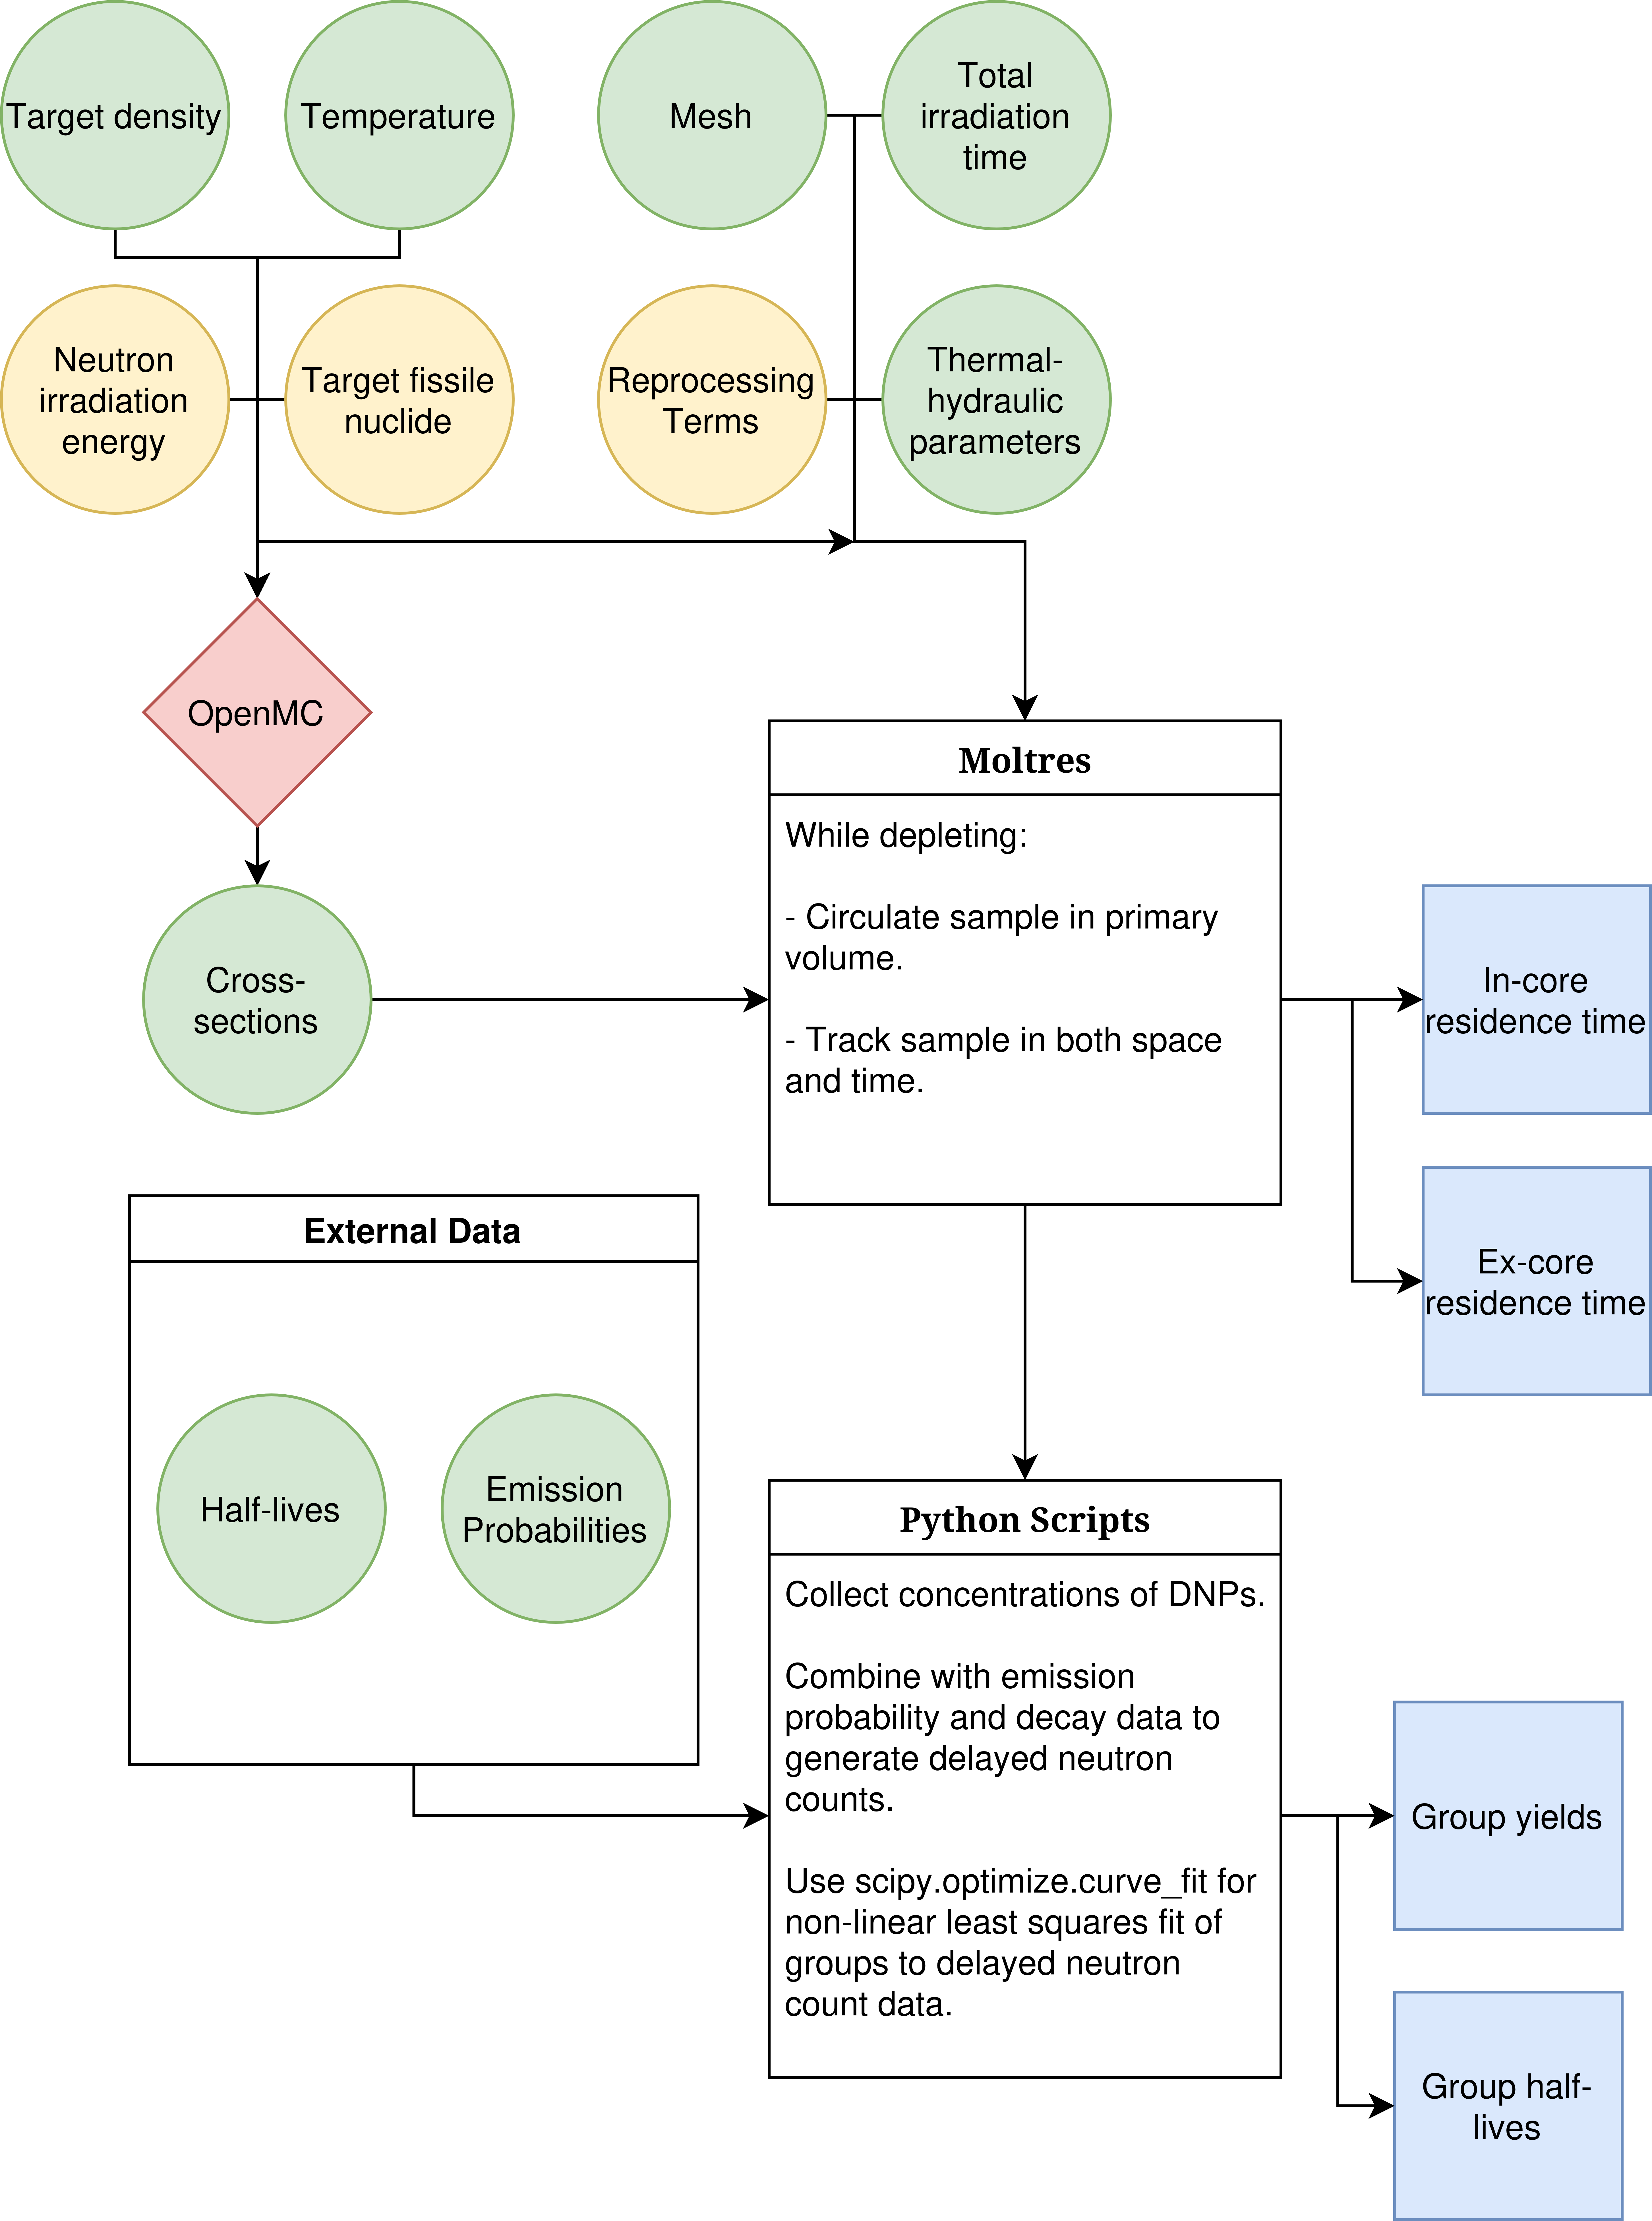
\includegraphics[width=0.9\linewidth]{images/sophisticated-model-4.png}
    \caption{Flow diagram of spatially resolved flow model used to generate flow-inclusive precursor group fit parameters.}
    \label{fig:sophisticated-model}
\end{figure}

There are two new parameters in the spatially resolved flow model that are not present in the 0D flow model.
The first is the mesh, which dictates the geometry of the problem.
MOOSE offers built-in meshing tools, though this may be insufficient depending on the complexity of the problem geometry.
In such a case, an external meshing tool, such as Gmsh, can be used \cite{geuzaine2009gmsh}.
The other new parameter is the thermal-hydraulics parameters.
This parameter captures many of the physical phenomena involved with inclusion of spatial resolution, as discussed in Section \ref{sec:moltres}.

The in-core and ex-core residence times are also outputs rather than inputs for the spatially resolved model.
This is because the residence times can be calculated from the movement of the irradiated sample over time in the fuel salt.
The in-core and ex-core residence times will change over time as the irradiated sample diffuses and mixes more in the fuel salt.
The net residence time, $\tau_{net}$, will not change over time without some change to the model such as an increased temperature difference or induced flow rate.
Equation \eqref{eq:incore-time} gives the in-core residence time as:

\begin{equation}
    \tau_{in} (t) = \frac{\int_{V_{in}} \int_{0}^t N(\vec{x}, t) dt d\vec{x}}{\int_{V} \int_{0}^t N(\vec{x}, t) dt d\vec{x}} \tau_{net},
    \label{eq:incore-time}
\end{equation}
where
\begin{align}
V_{in} &= \mbox{ the in-core volume} \nonumber \\
V &= \mbox{ the total primary volume } \nonumber \\
N(\vec{x}, t) &= \mbox{ the time and space resolved sample concentration} \nonumber \\
\tau_{net} &= \mbox{ the net residence, or circulation, time of the fuel salt.} \nonumber
\end{align}

The ex-core residence time can be calculated in the same way, or alternatively as shown in Equation \eqref{eq:excore-time} as:

\begin{equation}
    \tau_{ex} = \tau_{net} - \tau_{in}.
    \label{eq:excore-time}
\end{equation}

\section{Delayed Neutron Count Rate Generation}
\label{sec:delnu-counts}
Although the 0D flow model overview has been discussed, execution details were not.
The following sub-sections provide specific information on the methodology behind the OpenMC block.
This includes a detailed discussion on the concentrations generated by OpenMC and the data used with those concentrations to produce a delayed neutron count rate.


\subsection{Delayed Neutron Precursor Concentrations}
The OpenMC model uses a fixed-source problem on a three-gram spherical sample of a fissile target.
A uniformly distributed source is placed inside the target with a vacuum boundary condition at the edge of the sphere.
The sample must have a sufficiently large volume to ensure a high number of fissions, but excessive volume increases self-shielding and self-multiplication.
Adjusting the density mitigates this issue: higher density increases self-shielding and self-multiplication, while lower density reduces fission probability and worsens statistical accuracy.

The fixed-source in this model consists entirely of neutrons at a specific energy, rather than a spectrum.
This energy dictates fission cross sections, transmutation cross sections, and fission yields.
Traditionally, tabulated group parameter data is formatted for a single energy or energy range, such as fast or thermal.
However, macroscopic experiments, discussed in Section \ref{sec:measurementofdnps}, use reactors with varying neutron energy spectra, not mono-energetic neutrons.
This could be addressed by modeling a reactor in OpenMC and using a k-eigenvalue solve to generate a neutron energy spectrum.
However, this work assumes the spectral effects are sufficiently small to exclude.
Photons can also generate delayed neutrons through photofission, though this is not investigated here \cite{kinlaw2007delayed}.

The neutron source distribution does not replicate the experimental process, where neutrons irradiate the sample externally rather than internally.
However, an evenly distributed source eliminates self-shielding concerns.
The exact spatial locations of fission events within the sample should negligibly affect the nuclide concentrations, which are the outputs of the OpenMC simulation.
With a density of 10 $\frac{g}{cc}$, the spherical sample has a radius of approximately 0.4 $cm$.
The spatial resolution of concentrations within the sample is insignificant.
Additionally, the concentrations extracted from the OpenMC simulation are spatially collapsed in the post-processing, so the spatial effect of a uniformly distributed source serves only to reduce any self-shielding effects which could reduce the statistics and cause more transmutation than expected.

After running the OpenMC simulation, the concentrations are collected from the depletion results for the final irradiation time step.
These final concentrations are then converted into a delayed neutron count rate.

\subsection{Concentrations to Count Rate}
After receiving the concentrations from OpenMC, the concentrations of each nuclide as a function of time for the measurement period can be determined.
The concentrations are calculated as a function of half life, as shown in Equation \eqref{eq:radiodec} where the concentration as a function of time is:

\begin{equation}
    N(t) = N_0 e^{-\lambda t}.
    \label{eq:radiodec}
\end{equation}

This is a simple equation which does not take into account decay chains between nuclides.
An alternative approach which does account for these decay chains is to use repeated decay simulations of OpenMC in order to generate concentrations as a function of time.
These concentrations can be used at coarse time steps and linearly interpolated using SciPy, enabling the scripts to access these more accurate concentrations at any time after irradiation of the sample \cite{virtanen2020scipy}.
This approach does not account for particles generated during decay, as it is considered beyond the scope of this work \cite{chen2002rigorous}.
A comparison of these two approaches is investigated in Section \ref{sec:decaychaindaughters}.

The concentrations are combined with Equation \eqref{eq:delnu-exact}, recreated here:
\begin{equation}
n_d(t) = \epsilon \sum_{i=1}^{I} P_{n, i} \lambda_i N_{i}(t).
\nonumber
\end{equation}


The efficiency term, $\epsilon$, is set to 1 in this work, since the simulated method provides a count rate that includes every produced delayed neutron.
Each \gls{DNP} has its contribution over time summed up, generating the delayed neutron count rate.
%The delayed neutron count contribution over time is summed for each nuclide, generating the delayed neutron count rate.

\section{Delayed Neutron Precursor Group Reconstruction}
\label{sec:delnu-groups}

Once the delayed neutron count rate is generated, it is converted into \gls{DNP} group parameters.
Fitting the group parameters requires a non-linear least squares method, as both the group half-lives and yields must be determined.
The equation describing the problem appears in Equation \eqref{eq:delnu-fit}, recreated here:
\begin{equation}
\dot{n}_d(t) \approx \epsilon F_s \sum_{k=1}^{K}  \bar{\nu}_{d, k} \lambda_k e^{-\lambda_k t}.
\nonumber
\end{equation}

An important consideration for this process is the selection of time values for generating the group fits.
Increasing the number of time nodes raises computational costs, but too few nodes result in a poorer fit \cite{parish1999status}.
Section \ref{sec:time-eval} shows the sensitivity study for the time nodes, for both the node spacing and the maximum time to measure delayed neutrons.

Another consideration for the non-linear least squares solve is the covariance, which is larger for the pulse irradiation fit than for the saturation irradiation fit.
This results from multiplying the group yield by the group decay constant.
Attempts to replace this multiplication with an independent term produce poor fits, as the multiplication is not independent and is necessary for accurate modeling.

The non-linear least squares process also involves linearization and normalization of the data.
The normalization is handled by taking the delayed neutron count rate, dividing by the fission term \footnote{The fission term is either the net number of fissions or the fission rate, depending on the irradiation type.}, and taking the natural logarithm.
The normalized count rate is then passed into the non-linear least squares fitting.
The linearization is handled by taking the natural logarithm of the delayed neutron count rate.
This treatment reduces both the covariance and the $\chi^2$ of the fit.
Bounds from 0 to 1000 are set for each term to speed up the process, while convergence tolerances are set slightly above machine tolerance at $2.23 \times 10^{16}$ to ensure a well-refined solution.
The convergence criteria include changes in the independent variables and the norm of the gradient, with termination occurring when either criterion meets the set tolerance.


Sample self-multiplication, mentioned in Section \ref{sec:measurementofdnps}, is another consideration.
However, since the fission counts are taken directly from OpenMC tallies, self-multiplication is included and does not introduce error.

The final consideration in \gls{DNP} group reconstruction is uncertainty.
This work tracks uncertainties using the uncertainties package \cite{uncertaintiespackage}.
These uncertainties include uncertainties in cross sections, fission yields, half-lives, and emission probabilities.
These uncertainties are used in the $\chi^2$ minimization, as shown in Equation \eqref{eq:minthis}.


%\begin{description}
%    \item $t_f$ is the final time after irradiation, starting at $t=0$ immediately following irradiation
%    \item $b_t$ is the delayed neutron count vector at the row where the time value is $t$
%    \item $A_t$ is the coefficient matrix at the row where the time value is $t$
%    \item $x_t$ is the solution vector at the row where the time value is $t$
%\end{description}

Once the group fits and their uncertainties are generated, the final step to obtain the finalized group parameters is to combine the saturation and pulse irradiation results.
Saturation irradiation provides better statistics for longer-lived groups, while pulse irradiation is better for shorter-lived groups.
Brady combines the results by using four long-period groups from saturation irradiation and four short-period groups from pulse irradiation.
The groups are renormalized at the second group, where the two longest-lived group half-lives and yield ratios use the saturation results \cite{brady1988evaluation}.
The remaining groups use the pulse irradiation results.

This work uses a similar but slightly simplified approach.
The group parameters are first calculated for both pulse and saturation irradiation.
Then, the two longest-lived groups use the saturation irradiation results, while the four shortest-lived groups use the pulse irradiation results.


%\subsection{Group Concentrations from Nuclides}

%Fractional fitting (this is for running next Griffin/Pronghorn step)

%\section{Simulated Scenarios}

%\subsection{Verification}
%Comparison of Griffin/Pronghorn quasi-static to Moltres quasi-static to Moltres with fixed groups (old and new)

%\subsection{Validation}
%MSRE coastdown

%\subsection{Safeguards}
%Diversion scenario effects

%\subsection{Safety}
%Various safety transients



\chapter{Preliminary Results}

For the preliminary results, all possible variations in the input parameters are not resolved.
Instead, a default approach is utilized, with variations for refining the parameters.
Thermal fission of uranium-235 is used with the \gls{MSBR} reprocessing scheme with 10 second in-core and 10-second ex-core residence times at a temperature of 298.15 $K$ and a density of 10 grams per centimeter cubed irradiated over seven minutes with linearly spaced time nodes and decay daughter tracking for the group parameter non-linear least squares fit.

\section{Sensitivity Studies}
\label{sec:model-refinement}

\subsection{Constants for Simulations}

These sensitivity studies are used to analyze parameters that are held constant during the simulations and determine if simplifications can be made to some with negligible impact on the results.

\subsubsection{Temperature}

\subsubsection{Target Density}

\subsubsection{Total Irradiation Time}

\subsubsection{Total Decay Time and Decay Time Steps}
\label{sec:time-eval}
The bulk of the computational cost comes from writing statepoint files; sufficient resolution is required to ensure a smooth decay curve.

\subsubsection{Large Cycle Time Elements}
\label{sec:large-tcyc}

\subsubsection{Refuel Rate}
\label{sec:ref-rate}

\subsubsection{Decay Chain Parents}
\label{sec:decaychaindaughters}

\subsection{Variables for Simulations}

These sensitivity studies are used to analyze the parameters that change between simulations to understand the effect these changing parameters have on the results.

\subsubsection{Removal Rates}
\label{sec:repr-scale}

\subsubsection{In and Ex-core Residence Times}
\label{sec:res-time-var}

\subsubsection{Combined Removal Rates and Residence Times}

\section{Verification and Validation}

\subsection{0D Flow Model Verification}

Microscopic group parameters \cite{leconte2020new, mills1991study} should match static results (no flow or chemical removal.)

\subsection{0D Flow Model Validation}

MSRE pump start-up and coast-down with Moltres and Quasimolto \cite{prince1968zero, reynolds2023analysis}.

\chapter{Proposed Work}

\section{Develop Sophisticated Model}

Although the 0D flow model provides useful insights, it does not provide a high level of fidelity for any specific geometry.
To evaluate the accuracy of the 0D flow model, a spatially resolved model will be developed.
This model is key to determining if the 0D flow model produces \gls{DNP} group parameters of sufficient accuracy, and if not, then what the weakness are.
The spatially resolved model is discussed in detail in Section \ref{sec:soph-model}.

This spatially resolved model will be used in a comparison for multiple levels of fidelity of generating the \gls{DNP} group parameters: data only using cumulative fission yields, OpenMC simulations with depletion, spatially resolved using cumulative fission yields, and spatially resolved with depletion.
Each step up becomes more computationally expensive, so if a simpler method is able to generate \gls{DNP} group parameters with negligible differences, it will be used preferentially.

The process for comparing the 0D flow model and the spatially resolved model is as follows: the spatially resolved model runs and generates \gls{DNP} group parameters and residence times, the residence times are used to feed into the 0D flow model, the resulting \gls{DNP} group parameters are compared between the two models.
If the results match, then this would indicate that the 0D flow model only needs residence time data for a given \gls{MSR} to generate the \gls{DNP} group parameters.
If they do not match, then a spatially resolved approach will be necessary to properly generate the \gls{MSR} \gls{DNP} group parameters.

\section{Spatially Resolved Depletion Effects on Precursors}

Net delayed neutron yield; group abundances; group decays; comparison of most impactful nuclides (?)

Include polynomial fits (figures) showing how group parameters vary based on tabulated parameters (in-core, ex-core, chemical removal scaling, etc.)

Comparison with 0D Flow Model

\section{Resolve DNP Spectra}
The delayed neutron energy spectra, $\chi_d$ is important for accurate prediction of reactor kinetics \cite{das1993importance}.
This can be seen in the equation for the effective delayed neutron fraction in Equation \eqref{eq:betaeff-exact}, recreated here as:
\begin{equation}
    \beta_{eff} = \frac{\int \Phi^\dagger \chi_d \beta \bar{\nu} \Sigma_f \Phi \; dE d\vec{\Omega} d\vec{r}}{\int \Phi^\dagger \chi \bar{\nu} \Sigma_f \Phi \; dE d\vec{\Omega} d\vec{r}}.
    \nonumber
\end{equation}
The methodology to evaluate the delayed neutron spectra is discussed in Section \ref{sec:groupspectra}.

\section{Uncertainty Quantification}

\href{https://www.researchgate.net/publication/329403358_A_new_framework_for_sampling-based_uncertainty_quantification_of_the_six-group_reactor_kinetic_parameters}{Kozlowski paper}
Using sensitivity to flow and reprocessing.
Uncertainty in half lives and emission probabilities is small.
Neglect uncertainty in concentrations from OpenMC (cross sections, fission yields, half lives, transmutations, decay yields, etc.).

\section{Other extensions}
\begin{itemize}
\item Diffusion effect (not really modelable in time pulses only unless multiple materials are used) (could be approximated in 0D Flow Model).
\item Photoneutrons - investigate
\item Spatially resolved flux in 0D Flow Model - consider, Specific neutron spectra
\item Thermochemical effects - different nuclides will have different chemical removal rates, which will affect results (Sam knows more about this and could help me figure out if there would be something here in particular worth investigating)
\end{itemize}
\appendix
\chapter{Appendix A: Derivation of Simplfied Flowing Irradiation Delayed Neutron Counts for Equal Residence Times}
\renewcommand{\theequation}{A\thechapter.\arabic{equation}}
\label{ref:appendixA}
The delayed neutron count rate will be different in an \gls{MSR} than a stationary sample, as the sample is irradiated for the in-core residence time and not irradiated for the ex-core residence time.
The derivation presented in this appendix captures this effect.
This derivation begins with Equations \eqref{eq:wilson-R} and \eqref{eq:wilson-n} provided by Wilson and England \cite{wilson2002delayed}, modified to a single \gls{DNP} group $k$ as:
\begin{equation}
    R_k(t) = \bar{\nu}_{d, k} \lambda_k e^{-\lambda_k t},
    \label{eq:wilson-R}
\end{equation}
and
\begin{equation}
    \dot{n}_{d,k}(T, t) = \bar{\nu}_{d,k} \int_{0}^{T} F(\tau) R_k(T-\tau+t) d\tau,
    \label{eq:wilson-n}
\end{equation}
where
\begin{align}
K &= \text{ the number of \gls{DNP} groups $[\#]$} \nonumber \\
\bar{\nu}_{d,k} &= \text{ the group $k$ delayed neutron yield $[-]$} \nonumber \\
\lambda_k &= \text{ the group $k$ decay constant $[s^{-1}]$} \nonumber \\
T &= \mbox{ the duration of the fission history [$s$]} \nonumber \\
t &= \mbox{ the decay time from the end of the fission history [$s$]} \nonumber \\
\dot{n}_{d}(T, t) &= \text{ the delayed neutron count rate $[\# \cdot s^{-1}]$} \nonumber \\
R_k(t) &= \mbox{ the probability of delayed neutron emission from group $k$ at time $t$ $[\# \cdot s^{-1}]$} \nonumber \\
F(\tau) &= \mbox{ the fission rate history [$\frac{\#}{s}$].} \nonumber
\end{align}
Because the results are normalized to a single delayed neutron, the $\bar{\nu}_d$ term is divided out.

Although the saturation, or infinite, irradiation derivation makes use of assuming the time is infinite, due to the spatial dependence of this problem, the in-core and ex-core timing must be handled properly.
%For example, if the fission rate history uses a Fourier decomposition of a square wave, then it would not be possible to extract spatial information from this formulation.
%Specifically, it is important where in the primary loop the sample initially exists.
If the sample is initially in the core inlet, then the final portion of the fission rate history for each circulation must consist purely of decay.
If the sample is initially in the center of the core, then the final portion of the fission rate history for each circulation must consist of irradiation.

For this derivation, the sample is assumed to exist as a point at the core inlet.
It will circulate through the in-core region, then the ex-core region, and repeat until the net irradiation time $T$ has elapsed.
At that point, the delayed neutron count rate will be collected with $t$ starting at zero.
This means the irradiation consists of an in-core residence time of fission followed by an ex-core residence time of decay, after which the cycle repeats until the net irradiation time is met.
The normalized fission rate history is therefore given as a square wave composed of steps up and down:
\begin{align}
    \frac{F(\tau)}{F_0} = \sum_{j=0}^{J_{in}} \overbrace{H(\tau - j\cdot \tau_{net})}^\text{Step up} - \overbrace{H(\tau - j \cdot\tau_{net} -\tau_{in})}^\text{Step down},
    \label{eq:pos-square}
\end{align}
where
\begin{align}
    H =& \text{ the Heaviside function [-]} \nonumber \\
    \tau_{net} =& \;\tau_{in} + \tau_{ex} \nonumber \\
    =& \text{ the total time per circulation [$s$]} \nonumber \\
    J_{in} =& \left\lfloor \frac{T}{\tau_{net}} \right\rfloor \nonumber \\
     =& \text{ the number of times the sample enters the core minus one [$\#$]} \nonumber \\
    F_0 =& \text{ the magnitude of the constant fission rate [$\frac{\#}{s}$].} \nonumber
\end{align}
This function could be made to sum over infinity instead of $J_{in}$, since any Heaviside in which the value of $j \tau_{net}$ is larger than $T$ would become zero.
However, to make the equation cleaner, this clearer limit of $J_{in}$ is used.

Plugging this into Equation \eqref{eq:wilson-n} for group $k$ yields:
\begin{align}
\dot{n}_{d, k}(T, t) =& \int_{0}^{T} \sum_{j=0}^{J_{in}} H(\tau - j\cdot \tau_{net}) \bar{\nu}_{d, k} \lambda_k e^{-\lambda_k (T-\tau+t)} d\tau \nonumber\\
& - \int_{0}^{T} \sum_{j=0}^{J_{in}} H(\tau - j \cdot\tau_{net} - \tau_{in}) \bar{\nu}_{d, k} \lambda_k e^{-\lambda_k (T-\tau+t)} d\tau,
\end{align}
from which the common terms of $F_0$, $\bar{\nu}_{d, k}$, and $\lambda_k$ can be moved to the left-hand side:
\begin{align}
\frac{\dot{n}_{d, k}(T, t)}{F_0 \bar{\nu}_{d, k} \lambda_k} =& \int_{0}^{T} \sum_{j=0}^{J_{in}} H(\tau - j\cdot \tau_{net})   e^{-\lambda_k (T-\tau+t)} d\tau \nonumber\\
& - \int_{0}^{T} \sum_{j=0}^{J_{in}} H(\tau - j \cdot\tau_{net} - \tau_{in}) e^{-\lambda_k (T-\tau+t)} d\tau.
\end{align}

Solving the integrals yields:
\begin{align}
\frac{\dot{n}_{d, k}(T, t)}{F_0 \bar{\nu}_{d, k} \lambda_k} =& \sum_{j=0}^{J_{in}} \frac{H(T- j \cdot \tau_{net})}{\lambda_k} \left( e^{-\lambda_k t} - e^{-\lambda_k (t + T - j \cdot \tau_{net})} \right) \nonumber\\
& - \sum_{j=0}^{J_{in}} \frac{H(T- j \cdot \tau_{net} - \tau_{in})}{\lambda_k} \left( e^{-\lambda_k t} - e^{-\lambda_k (t + T - j \cdot \tau_{net} -  \tau_{in})} \right).
\end{align}
The Heaviside function in the first summation resolves to unity for every value of $j$ up to $J_{in}$, and is zero for any values of $j$ larger than $J_{in}$.
The second Heaviside is modified by $\tau_{in}$, so the limits of summation must be adjusted.
The problem becomes:
\begin{align}
\frac{\dot{n}_{d, k}(T, t)}{F_0 \bar{\nu}_{d, k}} =& \sum_{j=0}^{J_{in}} \left( e^{-\lambda_k t} - e^{-\lambda_k (t + T - j \cdot \tau_{net})} \right) \nonumber\\
& - \sum_{j=0}^{J_{ex}} \left( e^{-\lambda_k t} - e^{-\lambda_k (t + T - j \cdot \tau_{net} - \tau_{in})} \right),
\end{align}
where
\begin{align}
    J_{ex} =& \left\lfloor \frac{T-\tau_{in}}{\tau_{net}} \right\rfloor \nonumber \\
     =& \text{ the number of times the sample exits the core minus one [$\#$]} \nonumber
\end{align}
which, because $J_{ex}$ is always less than $J_{in}$, can be further simplified to:
\begin{align}
\frac{\dot{n}_{d, k}(T, t)}{F_0 \bar{\nu}_{d, k}} =& \sum_{j=0}^{J_{ex}} \left( e^{-\lambda_k t} - e^{-\lambda_k (t + T - j \cdot \tau_{net})} - e^{-\lambda_k t} + e^{-\lambda_k (t + T - j \cdot \tau_{net} - \tau_{in})} \right) \nonumber \\ &+ \sum_{j=J_{ex}+1}^{J_{in}} \left( e^{-\lambda_k t} - e^{-\lambda_k (t + T - j \cdot \tau_{net})} \right).
\end{align}
The exponential terms can be moved outside of the summations:
\begin{align}
\frac{\dot{n}_{d, k}(T, t)}{F_0 \bar{\nu}_{d, k}} &= e^{-\lambda_k t} \sum_{j=0}^{J_{ex}} \left( e^{-\lambda_k (T - \tau_{in} - j \cdot \tau_{net})} - e^{-\lambda_k (T - j \cdot \tau_{net})}  \right) \nonumber \\ &+ e^{-\lambda_k t} \sum_{j=J_{ex}+1}^{J_{in}} \left( 1 - e^{-\lambda_k (T - j \cdot \tau_{net})} \right).
\label{eq:sumform}
\end{align}

The closed form of the geometric series can be calculated, which enables the summation terms to collapse and be written as:
\begin{align}
    \frac{\dot{n}_{d, k}(T, t)}{F_0 \bar{\nu}_{d, k}} =& e^{-\lambda_kt} \left( \left(J_{in}-J_{ex}\right) + \frac{e^{-\lambda_kT}}{d-1}  \left( e^{\lambda_k\tau_{in}}d^{J_{ex}+1} - e^{\lambda_k\tau_{in}} + 1 - d^{J_{in}+1} \right) \right),
\end{align}
where
\begin{align}
    d &= e^{\lambda_k\tau_{net}}
\end{align}

\begin{comment}
\begin{equation}
    \frac{\dot{n}_{d, k}(T, t)}{F_0 \bar{\nu}_{d, k}} = \sum_{j=0}^{{J}}\left(\left(e^{-\lambda_k\cdot\left(t+T-j\cdot \tau_{net}\right)}\right)\cdot\left(e^{\left(\lambda_k\cdot \tau_{in}\right)}-1\right)\right)
\end{equation}
\end{comment}

If the net irradiation time $T$ is infinite and the ex-core residence time is zero, then the delayed neutron count rate simplifies to:
\begin{align}
\dot{n}_{d, k}(T, t) =& F_0 \bar{\nu}_{d, k} e^{-\lambda_k t},
\label{eq:wilseng-examp}
\end{align}
which matches the result from Wilson and England \cite{wilson2002delayed}.
%However, for non-zero ex-core residence times, the results do not match, which is expected.
%However, as previously mentioned, this infinite approach will not work for the spatially dependent analysis.
However, for cases with non-zero ex-core residence times, the behavior is noticeably different.
For example, if an in-core residence time $\tau_{in}$ is selected which is relatively small compared to the ex-core residence time $\tau_{ex}$, Equation \eqref{eq:wilseng-examp} would not vary at all, even though the fission rate history would be significantly different.
By isolating the delayed neutron count rate $\dot{n}_{d,k}$ and summing over all $K$ groups, the finalized equation can be formulated as:
\begin{align}
\dot{n}_{d}(T, t) =F_0 \sum_{k=1}^K \bar{\nu}_{d, k} e^{-\lambda_kt} \left( \left(J_{in}-J_{ex}\right) - \frac{e^{-\lambda_kT}}{1-d}  \left( e^{\lambda_k\tau_{in}}d^{J_{ex}+1} - e^{\lambda_k\tau_{in}} + 1 - d^{J_{in}+1} \right) \right).
\end{align}
This equation is not stable for all in-core and ex-core residence times, and is unstable if the ex-core time goes to zero.
The summation form given in Equation \eqref{eq:sumform} is stable for general problems.
The summation form is similar to the form presented by Wilson and England for an arbitrary irradiation time:
\begin{equation}
    \dot{n}_{d}(T, t) = F_0 \sum_{k=1}^K \bar{\nu}_{d, k} e^{-\lambda_k t} \left( 1 - e^{-\lambda_k T}\right)
\end{equation}
If the in-core residence time is zero, then the delayed neutron count rate goes to zero, which is the expected behavior.



\begin{comment}
\todo{test $\tau_{in}=0$}
\begin{align}
\dot{n}_{d, k}(T, t) =& F_0 \bar{\nu}_{d, k} e^{-\lambda_k t} \left(1 - e^{-\lambda_k T} +  \left( 1-e^{\lambda_k \tau_{ex}} \right) \sum_{j=1}^J e^{\lambda_k (j \cdot \tau_{in} + j \cdot \tau_{ex} - \tau_{ex}-T)} \right)
\end{align}

\begin{align}
\dot{n}_{d, k}(T, t) =& F_0 \bar{\nu}_{d, k} e^{-\lambda_k t} \left(1 - e^{-\lambda_k T} +  \left( 1-e^{\lambda_k \tau_{ex}} \right) \sum_{j=1}^J e^{\lambda_k (j \cdot \tau_{ex} - \tau_{ex}-T)} \right)
\end{align}

\begin{align}
\dot{n}_{d, k}(T, t) =& F_0 \bar{\nu}_{d, k} e^{-\lambda_k t} \left(1 - e^{-\lambda_k T} +  \left( 1-e^{\lambda_k \tau_{ex}} \right) ( e^{-\lambda_k T} + e^{\lambda_k (\tau_{ex} -T)} + e^{\lambda_k (2 \tau_{ex} -T)} ...) \right)
\end{align}

Let $T=n\tau_{ex}$
\begin{align}
\dot{n}_{d, k}(T, t) =& F_0 \bar{\nu}_{d, k} e^{-\lambda_k t} \left(1 - e^{-\lambda_k n\tau_{ex}} +  \left( 1-e^{\lambda_k \tau_{ex}} \right) ( e^{-\lambda_k n\tau_{ex}} + e^{-\lambda_k ((n-1)\tau_{ex})} + e^{-\lambda_k ( (n-2)\tau_{ex})} ...) \right)
\end{align}

\begin{align}
\dot{n}_{d, k}(T, t) =& e^{-\lambda_k t} \left(1 - e^{-\lambda_k n\tau_{ex}} +  \left( 1-e^{\lambda_k \tau_{ex}} \right) ( e^{-\lambda_k n\tau_{ex}} + e^{-\lambda_k ((n-1)\tau_{ex})} + e^{-\lambda_k ( (n-2)\tau_{ex})} ...) \right)
\end{align}
\end{comment}




\backmatter

\bibliographystyle{apalike}
\bibliography{bibliography}

\end{document}
\endinput
%%
%% End of file `thesis-ex.tex'.
